\documentclass{article}

% packages
\usepackage{amsmath, amsthm, thmtools, amsfonts, amssymb, luacode, catchfile, tikzducks, hyperref, ifthen}
\ifcsname c@kobocompile\endcsname
	\usepackage[a5paper, total={1072pt, 1448pt}, margin=10pt, includeheadfoot]{geometry} % set page margins
\else
	\usepackage[a4paper, margin=50pt, includeheadfoot]{geometry}
\fi
\usepackage[shortlabels]{enumitem}
\usepackage[skip=3pt, indent=0pt]{parskip}

% language
\usepackage[bidi=basic, layout=tabular, provide=*]{babel}
\ifcsname c@english\endcsname
	\babelprovide[main, import]{english}
\else
	\babelprovide[main, import]{hebrew}
	\babelprovide{rl}
\fi
%\babelfont{rm}{Libertinus Serif}
\babelfont{rm}[Renderer=Harfbuzz]{Libertinus Serif}
\babelfont{sf}{Libertinus Sans}
\babelfont{tt}{Libertinus Mono}

% style
\AddToHook{cmd/section/before}{\clearpage}	% Add line break before section
\linespread{1.3}
\setcounter{secnumdepth}{0}		% Remove default number tags from sections, this won't do well with theorems
\AtBeginDocument{\setlength{\belowdisplayskip}{3pt}}
\AtBeginDocument{\setlength{\abovedisplayskip}{3pt}}
\graphicspath{ {../images/} }

% operators
\DeclareMathOperator\cis{cis}
\DeclareMathOperator\Sp{Sp}
\DeclareMathOperator\tr{tr}
\DeclareMathOperator\im{Im}
\DeclareMathOperator\re{Re}
\DeclareMathOperator\diag{diag}
\DeclareMathOperator*\lowlim{\underline{lim}}
\DeclareMathOperator*\uplim{\overline{lim}}
\DeclareMathOperator\rng{rng}
\DeclareMathOperator\Sym{Sym}
\DeclareMathOperator\Arg{Arg}
\DeclareMathOperator\Log{Log}
\DeclareMathOperator\dom{dom}
\DeclareMathOperator\supp{Supp}
\DeclareMathOperator\var{Var}
\DeclareMathOperator\cov{Cov}

% commands
%\renewcommand\qedsymbol{\textbf{מש''ל}}
%\renewcommand\qedsymbol{\fbox{\emoji{lizard}}}
\newcommand{\Aa}[0]{\mathcal{A}}
\newcommand{\Bb}[0]{\mathcal{B}}
\newcommand{\CC}[0]{\mathbb{C}}
\newcommand{\Cc}[0]{\mathcal{C}}
\newcommand{\EE}[0]{\mathbb{E}}
\newcommand{\FF}[0]{\mathbb{F}}
\newcommand{\Ff}[0]{\mathcal{F}}
\newcommand{\Ii}[0]{\mathcal{I}}
\newcommand{\Gg}[0]{\mathcal{G}}
\newcommand{\Ll}[0]{\mathcal{L}}
\newcommand{\Mm}[0]{\mathcal{M}}
\newcommand{\NN}[0]{\mathbb{N}}
\newcommand{\Nn}[0]{\mathcal{N}}
\newcommand{\PP}[0]{\mathbb{P}}
\newcommand{\Pp}[0]{\mathcal{P}}
\newcommand{\QQ}[0]{\mathbb{Q}}
\newcommand{\RR}[0]{\mathbb{R}}
\newcommand{\Rr}[0]{\mathcal{R}}
\newcommand{\Ss}[0]{\mathcal{S}}
\newcommand{\TT}[0]{\mathbb{T}}
\newcommand{\Uu}[0]{\mathcal{U}}
\newcommand{\Vv}[0]{\mathcal{V}}
\newcommand{\Ww}[0]{\mathcal{W}}
\newcommand{\ZZ}[0]{\mathbb{Z}}
\newcommand{\acts}[0]{\circlearrowright}
\newcommand{\explain}[2] {
	\begin{flalign*}
		 && \text{#2} && \text{#1}
	\end{flalign*}
}
\newcommand{\maketitleprint}[0]{ \begin{center}
	%\begin{tikzpicture}[scale=3]
	%	\duck[graduate=gray!20!black, tassel=red!70!black]
	%\end{tikzpicture}	
	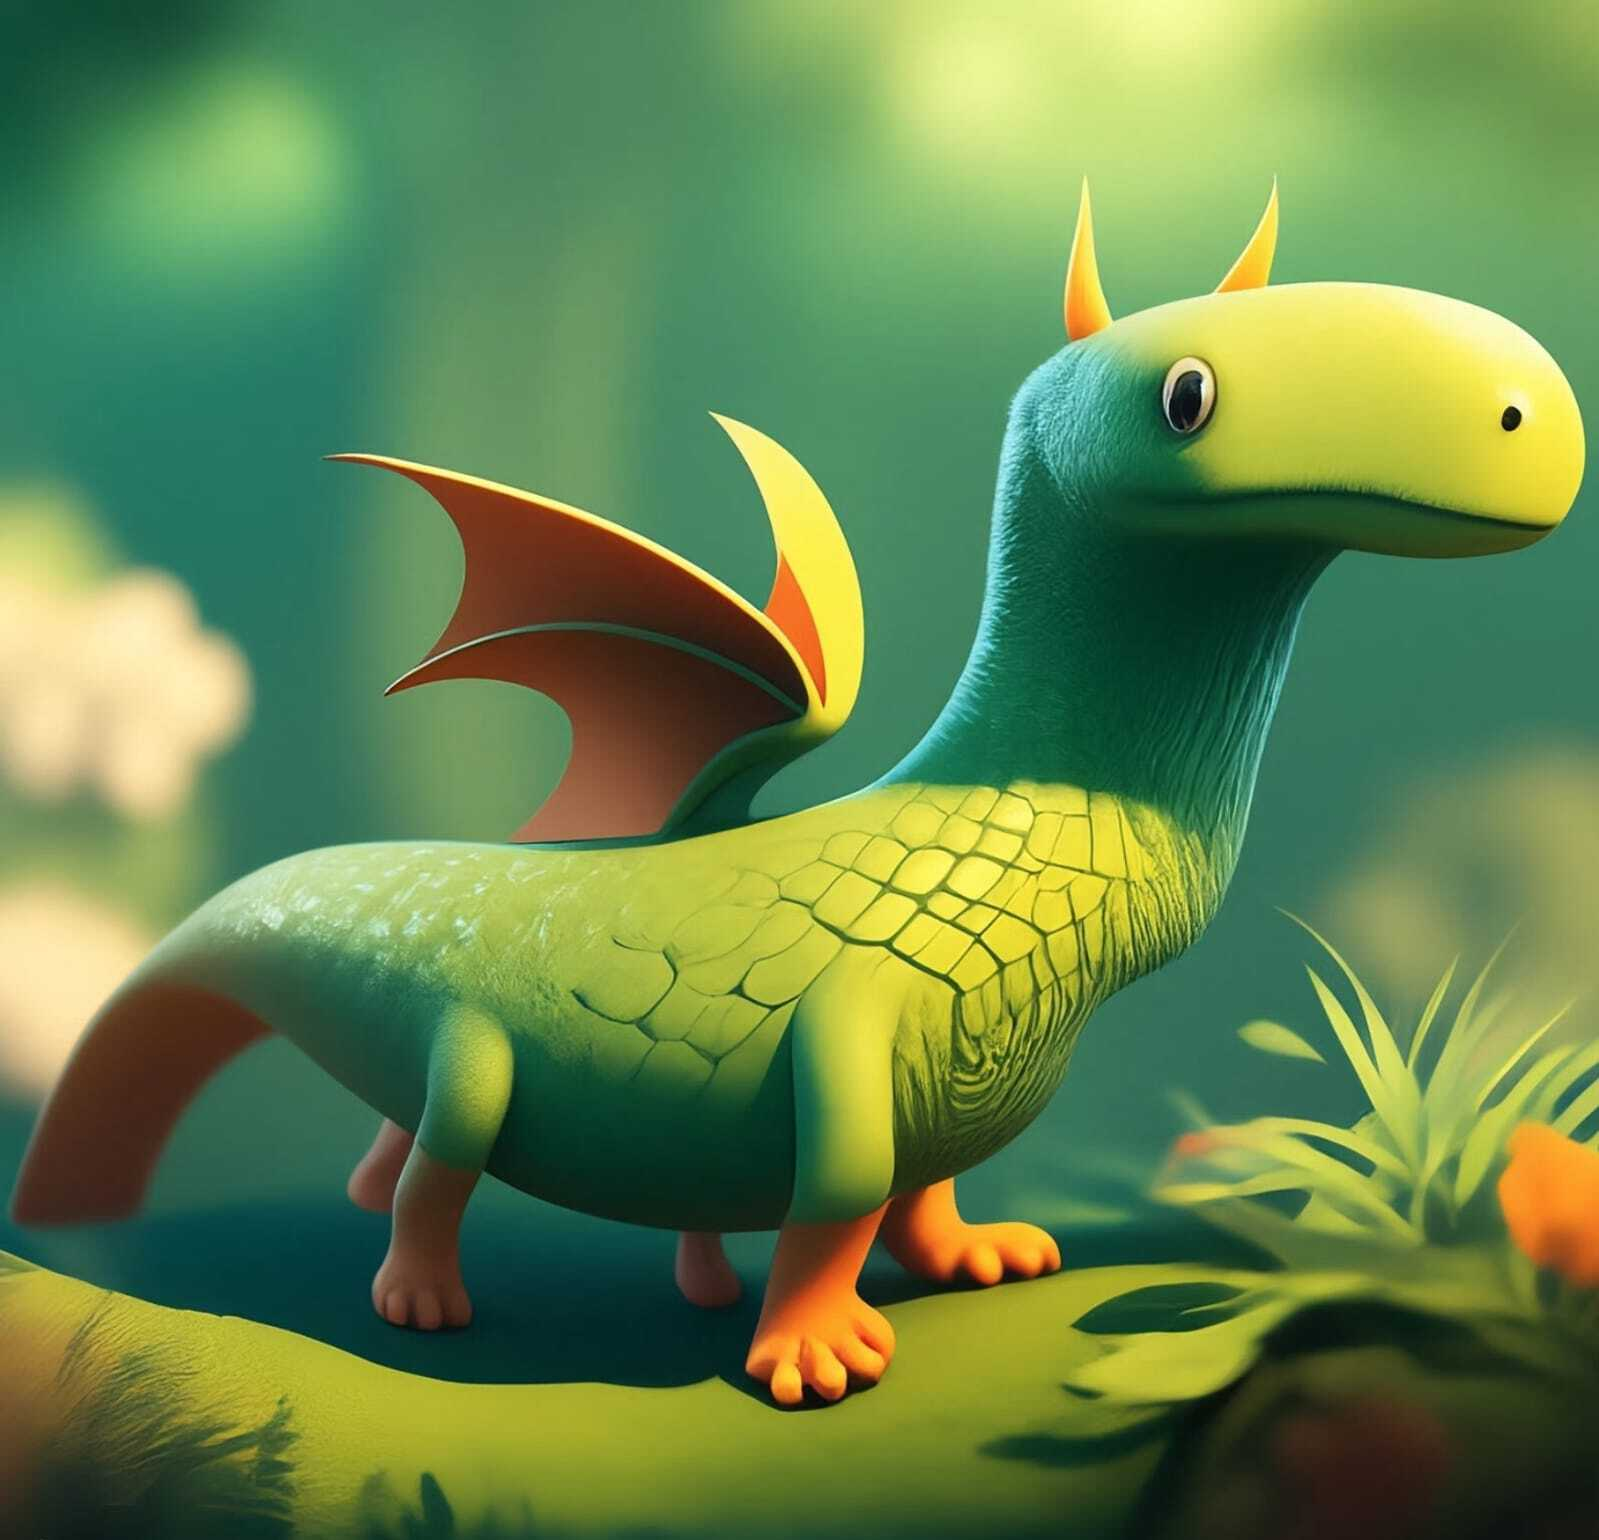
\includegraphics[width=6cm]{cover}
\end{center}
}

% theorem commands
\newtheoremstyle{c_remark}
	{}	% Space above
	{}	% Space below
	{}% Body font
	{}	% Indent amount
	{\bfseries}	% Theorem head font
	{}	% Punctuation after theorem head
	{.5em}	% Space after theorem head
	{\thmname{#1}\thmnumber{ #2}\thmnote{ \normalfont{\text{(#3)}}}}	% head content
\newtheoremstyle{c_definition}
	{3pt}	% Space above
	{3pt}	% Space below
	{}% Body font
	{}	% Indent amount
	{\bfseries}	% Theorem head font
	{}	% Punctuation after theorem head
	{.5em}	% Space after theorem head
	{\thmname{#1}\thmnumber{ #2}\thmnote{ \normalfont{\text{(#3)}}}}	% head content
\newtheoremstyle{c_plain}
	{3pt}	% Space above
	{3pt}	% Space below
	{\itshape}% Body font
	{}	% Indent amount
	{\bfseries}	% Theorem head font
	{}	% Punctuation after theorem head
	{.5em}	% Space after theorem head
	{\thmname{#1}\thmnumber{ #2}\thmnote{ \text{(#3)}}}	% head content

\ifcsname c@english\endcsname
	\theoremstyle{plain}
	\newtheorem{theorem}{Theorem}[section]
	\newtheorem{lemma}[theorem]{Lemma}
	\newtheorem{proposition}[theorem]{Proposition}
	\newtheorem*{proposition*}{Proposition}
	%\newtheorem{corollary}[theorem]{אין חלופה עברית}

	\theoremstyle{definition}
	\newtheorem{definition}[theorem]{Definition}
	\newtheorem*{definition*}{Definition}
	\newtheorem{example}{Example}[section]
	\newtheorem{exercise}{Exercise}[section]

	\theoremstyle{remark}
	\newtheorem*{remark}{Remark}
	\newtheorem*{solution}{Solution}
	\newtheorem{conclusion}[theorem]{Conclusion}
	\newtheorem{notation}[theorem]{Notation}
\else
	\theoremstyle{c_plain}
	\newtheorem{theorem}{משפט}[section]
	\newtheorem{lemma}[theorem]{למה}
	\newtheorem{proposition}[theorem]{טענה}
	\newtheorem*{proposition*}{טענה}
	%\newtheorem{corollary}[theorem]{אין חלופה עברית}

	\theoremstyle{c_definition}
	\newtheorem{definition}[theorem]{הגדרה}
	\newtheorem*{definition*}{הגדרה}
	\newtheorem{example}{דוגמה}[section]
	\newtheorem{exercise}{תרגיל}[section]

	\theoremstyle{c_remark}
	\newtheorem*{remark}{הערה}
	\newtheorem*{solution}{פתרון}
	\newtheorem{conclusion}[theorem]{מסקנה}
	\newtheorem{notation}[theorem]{סימון}
\fi

% Questions related commands
\newcounter{question}
\setcounter{question}{1}
\newcounter{sub_question}
\setcounter{sub_question}{1}

\ifcsname c@english\endcsname
	\newcommand{\question}[1][0]{
		\ifthenelse{#1 = 0}{}{\setcounter{question}{#1}}
		\section{Question \arabic{question}}
		\addtocounter{question}{1}
		\setcounter{sub_question}{1}
	}

	\newcommand{\subquestion}[1][0]{
		\ifthenelse{#1 = 0}{}{\setcounter{sub_question}{#1}}
		\subsection{Part \alph{sub_question}}
		\addtocounter{sub_question}{1}
	}
\else
	\newcommand{\question}[1][0]{
		\ifthenelse{#1 = 0}{}{\setcounter{question}{#1}}
		\section{שאלה \arabic{question}}
		\addtocounter{question}{1}
		\setcounter{sub_question}{1}
	}

	\newcommand{\subquestion}[1][0]{
		\ifthenelse{#1 = 0}{}{\setcounter{sub_question}{#1}}
		\subsection{סעיף \localecounter{letters.gershayim}{sub_question}}
		\addtocounter{sub_question}{1}
	}
\fi

% import lua and start of document
\directlua{common = require ('../common')}

\GetEnv{AUTHOR}

% headers
\author{\AUTHOR}
\date\today

\title{אנליזה פונקציונלית --- סיכום}
\setcounter{secnumdepth}{2}

\usepackage{fancyhdr}
\pagestyle{fancy}
\renewcommand{\headrulewidth}{0pt}

\begin{document}
\maketitle
\maketitleprint[teal]

\tableofcontents

\section{שיעור 1 --- 26.3.2025}
\subsection{רקע}
אנליזה פונקציונלית היא כמו אלגברה לינארית.
בקורס זה נחקור מרחבים וקטוריים והעתקות עליהם, אבל על מרחבים מורכבים יותר והעתקות מורכבות יותר.
נתחיל בשאלה,
\begin{exercise}
	יהי $(X, \rho)$ מרחב מטרי כלשהו, ונניח ש־$A \subseteq X$.
	נניח גם ש־${(a_n)}_{n = 1}^\infty \subseteq A$. \\
	מהם התנאים ההכרחיים על $A$ כך ש־$(a_n)$ תכלול תת־סדרת קושי?
\end{exercise}
נעבור לדוגמה וטענות מאינפי 1 לרענן את זכרוננו.
\begin{example}
	המרחב המטרי הכי אינטואיטיבי הוא $X = \RR$ ו־$\rho(x, y) = |x - y|$.
\end{example}
\begin{proposition}
	תהי $A \subseteq \RR$ כך ש־$A$ חסומה, ותהי ${(a_n)}_{n = 1}^\infty \subseteq A$,
	אז יש ל־$(a_n)$ תת־סדרת קושי.
\end{proposition}
\begin{proof}
	$A \subseteq [-R, R]$ עבור $R \in \RR$.
	נתחיל בהגדרה של $\Delta_0 = A$ ולכן יש אינסוף, ולכן יש בקטע $\Delta_0$ אינסוף נקודות של הסדרה, וכן $|\Delta_0| = 2R$.
	נבחן את הקטעים החוצים את $\Delta_0$, הם $[-R, 0], [0, R]$, נבחר את זה מביניהם שמכיל אינסוף נקודות של $(a_n)$ להיות $\Delta_1$, וכך נמשיך ונגדיר סדרה $(\Delta_n)$.
	נובע שהסדרה הנתונה היא סדרה יורדת, במובן ש־$\Delta_0 \supset \Delta_1 \supset \Delta_2 \supset \dots$, מתקיים גם $|\Delta_n| = \frac{|\Delta_0|}{2^n}$ לכל $n \in \NN$, ובכל $\Delta_n$ יש אינסוף נקודות של $(a_n)$.
	נבחר $a_{n_1} \in \Delta_1$ וכך באופן כללי גם $a_{n_k} \in \Delta_k$, לכן נובע $|a_{n_k} - a_{n_l}| \le \frac{1}{2^k}$ עבור $l \ge k$.
	לכן נובע שאכן ישנה תת־סדרת קושי בסדרה $(a_n)$.
\end{proof}
\begin{remark}
	טענה זו נכונה גם כאשר מסתכלים על מרחב $(\RR^n, \rho)$ עבור $\rho(x, y) = \sqrt{\sum_{i = 1}^{n} {(x_i - y_i)}^2}$.
\end{remark}
\begin{definition}[מרחב נורמי]
	יהי $V$ מרחב וקטורי מעל $\FF$ עבור $\FF \in \{ \RR, \CC \}$, ותהי פונקציה $\lVert \cdot \rVert : V \to \RR_{\ge0}$ המקיימת,
	\begin{enumerate}
		\item $x = 0_V \iff \lVert x \rVert = 0$
		\item $\forall \alpha \in \FF, \lVert \alpha x \rVert = |\alpha| \cdot \lVert x \rVert$
		\item $\forall x, y \in V, \lVert x + y \rVert \le \lVert x \rVert + \lVert y \rVert$
	\end{enumerate}
	אז $(V, \lVert \cdot \rVert)$ יקרא מרחב נורמי עם נורמה $\lVert \cdot \rVert$.
\end{definition}
\begin{definition}[מרחב l2]
	נגדיר את הקבוצה $l_2 = \{ x = (x_1, \dots) \mid \forall k \in \NN, x_k \in \RR, \sum_{i = 1}^{\infty} x_i^2 < \infty \}$.
	נגדיר גם,
	\[
		\lVert x \rVert = {\left(\sum_{i = 1}^{\infty} x_i^2\right)}^{\frac{1}{2}}
	\]
	אז המרחב הנורמי $l_2$ הוא הקבוצה והנורמה הללו.
\end{definition}
נבחין כי עלינו להוכיח שזהו אכן מרחב נורמי לפי ההגדרה.
\begin{theorem}[אי־שוויון קושי־שווארץ]
	מתקיים,
	\[
		\sum_{i = 1}^{n} |x_i| \cdot |y_i|
		\le {\left( \sum_{i = 1}^{n} x_i^2 \right)}^{\frac{1}{2}} \cdot {\left( \sum_{i = 1}^{n} y_i^2 \right)}^{\frac{1}{2}}
	\]
\end{theorem}
\begin{notation}
	נסמן $\langle x, y \rangle = \sum_{i = 1}^{n}  x_i y_i$.
\end{notation}
\begin{proof}
	עבור $t \in \FF$ סקלר כלשהו,
	\[
		0
		\le \langle x + ty, x + ty \rangle
		= \langle x, x \rangle + 2t \langle x, y \rangle + \langle y, y \rangle t^2
	\]
	עובדה ידועה היא $At^2 + Bt + C \ge 0 \implies B^2 - 4AC \le 0$ ולכן,
	\[
		{\left( \sum_{i = 1}^{n} x_i y_i \right)}^2
		\le {\left( \sum_{i = 1}^{n} x_i^2 \right)} \cdot {\left( \sum_{i = 1}^{n} y_i^2 \right)}
	\]
	ולכן,
	\[
		\left\lvert \sum_{i = 1}^{n} x_i y_i \right\rvert
		\le {\left( \sum_{i = 1}^{n} x_i^2 \right)}^{1/2} \cdot {\left( \sum_{i = 1}^{n} y_i^2 \right)}^{1/2}
	\]
	ואם נגדיר $x_i' = |x_i|$ וכן $y_i' = |y_i|$ אז מאי־השוויון הנתון נובע,
	\[
		\sum_{i = 1}^{n} |x_i'| \cdot |y_i'|
		\le {\left( \sum_{i = 1}^{n} x_i^2 \right)}^{\frac{1}{2}} \cdot {\left( \sum_{i = 1}^{n} y_i^2 \right)}^{\frac{1}{2}}
	\]
\end{proof}
נעבור להוכחת ההגדרה של $l_2$, כלומר ההוכחה שהנורמה שהגדרנו היא אכן נורמה.
\begin{proof}
	\begin{align*}
		{\lVert x + y \rVert}^2
		& = \sum_{i = 1}^{\infty} {(x_i + y_i)}^2 \\
		& = \sum_{i = 1}^{\infty} x_i^2 + 2 \sum_{i = 1}^{\infty} x_i y_i + \sum_{i = 1}^{\infty} y_i^2 \\
		& \le {\lVert x\rVert}^2 + 2 \lVert x \rVert \cdot \lVert y \rVert + {\lVert y \rVert}^2 \\
		& = {(\lVert x \rVert + \lVert y \rVert)}^2 \\
		& \implies \lVert x + y \rVert \le \lVert x \rVert + \lVert y \rVert
	\end{align*}
\end{proof}
עתה משקיבלנו ש־$l_2$ הוא אכן מרחב נורמי, נוכל לדון בתכונותיו.
\begin{example}
	במרחב $(l_2, \lVert \cdot \rVert)$ נגדיר את שפת כדור היחידה במרחב,
	\[
		S = \{ x \in l_2 \mid \lVert x \rVert = 1 \}
	\]
	נבחין כי $S$ קבוצה חסומה ב־$l_2$.
	נבחר ${(l_n)}_{n = 1}^\infty$ המוגדרת על־ידי $l_n = (0, \dots, 1, \dots)$ כאשר $l_n^n = 1, l_n^m = 0$ לכל $m \ne n$.
	כמובן מתקיים $\lVert l_n \rVert = 1$ לכל $n \in \NN$, ולכן סדרת הנקודות חסומה ב־$S$.
\end{example}
\begin{proposition}
	${(l_n)}_{n = 1}^\infty \subseteq l_2$ איננה כוללת תת־סדרת קושי.
\end{proposition}
\begin{proof}
	נבחין כי $\lVert l_n - l_m \rVert = \sqrt{2}$ לכל $n \ne m$.
\end{proof}
\begin{notation}[כדור]
	עבור מרחב מטרי $(X, \rho)$, נסמן $B_r(x) = \{ x \in X \mid \rho(x, x_0) < r \}$.
\end{notation}
\begin{definition}[קבוצה חסומה לחלוטין]
	יהי מרחב מטרי $(X, \rho)$ מרחב מטרי ותהי $A \subseteq X$, אז נאמר ש־$A$ חסומה לחלוטין (Totally bounded) אם לכל $\epsilon > 0$ קיים מספר סופי של נקודות $\{ x_1, \dots, x_N \} \subseteq X$,
	כך שמתקיים $A \subseteq \bigcup_{i = 1}^N B_\epsilon(x_i)$.
\end{definition}
מיד נראה שימוש בהגדרה זו במשפט, ובכך ניתן הצדקה להגדרה הלכאורה משונה הזאת.
\begin{theorem}[שקילות לחסימות לחלוטין]\label{totally_bounded_set_equivalecy_theorem}
	יהי מרחב מטרי $(X, \rho)$ ותהי $A \subseteq X$, אז התנאים הבאים שקולים,
	\begin{enumerate}
		\item $A$ חסומה לחלוטין.
		\item בכל סדרה של $A$ ניתן לבחור תת־סדרת קושי.
	\end{enumerate}
\end{theorem}
משפט זה הוא משפט חשוב ומרכזי, ועל הקורא לשנן את הוכחתו. את ההוכחה אומנם נראה בהרצאות הבאות, אך נראה עתה שימושים למשפט זה.
נעבור למשפט פחות חשוב ומרכזי,
\begin{theorem}[שקילות חסימות במרחבים האוקלידיים]
	נניח ש־$X = \RR^m$, וכן ש־$\rho(x, y) = \sqrt{\sum_{i = 1}^{m} {(x_i - y_i)}^2}$, אז אם $A \subseteq \RR^m$ חסומה, אז היא חסומה לחלוטין.
\end{theorem}
\begin{proof}
	נחסום את $A$ על־ידי קובייה מספיק גדולה, נחלק את הקובייה לתת־קוביות מספיק קטנות (ההצדקה מגיעה מאינפי 3), ונוכל לחסום כל קובייה כזו בכדור.
	נסמן $\{ x_i \} \subseteq \RR^m$ את מרכזי הקוביות ונקבל $A \subseteq \bigcup_{j = 1}^N B_\epsilon(x_j)$ מהגדרת החלוקה של הקובייה החוסמת.
\end{proof}
\begin{proposition}
	ב־$(l_2, \lVert \cdot \rVert)$ נגדיר את הקבוצה,
	\[
		\Pi = \{ x = (x_1, \dots) \in l_2 \mid \forall i \in \NN, |x_i| \le \frac{1}{2^{i - 1}} \}
	\]
	אם $x \in \Pi$ אז $\sum_{n = 1}^{\infty} x_n^2 < \infty$, ובהתאם בהכרח $\Pi \subseteq l_2$. \\
	הקבוצה $\Pi$ חסומה לחלוטין.
\end{proposition}
\begin{proof}
	תהי $(x_1, \dots) \in \Pi$, ונגדיר $x_n^* = (x_1, \dots, x_n, \dots, 0, 0, \dots)$.
	נגדיר גם $\Pi^*_n = \{ x = (x_1, \dots, x_n, 0, \dots) \mid |x_n| \le \frac{1}{2^{n - 1}} \}$.
	הקבוצה $\Pi_n^*$ חסומה לחלוטין, זאת שכן הקבוצה שקולה לקבוצה ב־$\RR^n$, ונבחין כי היא חסומה, ולכן ההוכחה שראינו קודם עודנה תקפה ובהתאם $\Pi_n^*$ חסומה לחלוטין. \\
	נבחין כי
	\[
		{\lVert x - x_n^* \rVert}^2
		= \sum_{i = n + 1}^{\infty} x_i^2
		\le \sum_{i = n + 1}^{\infty} \frac{1}{2^{2i - 2}}
		= \sum_{i = n + 1}^{\infty} \frac{4}{4^i}
		= \frac{1}{4^n} \cdot \frac{1}{1 - \frac{1}{4}}
		= \frac{1}{3 \cdot 4^{n - 1}}
	\]
	ולכן $\lVert x - x_n^* \rVert \le \frac{1}{2^{n - 1}}$.
	יהי $\epsilon > 0$, אז $\Pi_n^*$ חסומה לחלוטין ולכן קיימים $y^1, \dots, y^n \in l_2$ כך שמתקיים,
	\[
		\Pi_n^* \subseteq \bigcup_{i = 1}^N B_\epsilon(y^i)
	\]
	מצאנו שלכל $x_n^*$ ובכלל לכל $n$ קיים $i$ כך ש־$x_n^* \in B_{\epsilon}(y^i)$,
	עד כה עבדנו עם $n$ כללי, עתה נניח ש־$n$ מספיק גדול כך שיתקיים, $\lVert x - x_n^* \rVert < \epsilon$, כתוצאה מאי־השוויון שמצאנו לעיל.
	אז,
	\[
		\lVert x - y^i \rVert
		\le \lVert x - x_n^* \rVert + \lVert x_n^* - y^i \rVert
		< 2 \epsilon
	\]
	נובע ש־$\Pi \subseteq \bigcup_{i = 1}^N B_{2\epsilon}(y^i)$.
\end{proof}
נבחין כי עתה ראינו שב־$l_2$ במרחב נורמי יש קבוצות חסומות, זהו אכן מרחב מעניין.

\section{שיעור 2 --- 2.4.2025}
\subsection{חסימות לחלוטין}
נראה את הוכחתם של שני משפטים שמומלץ לזכור.
המשפט הראשון הוא משפט\ \ref{totally_bounded_set_equivalecy_theorem}, בקורס זה נקרא לו משפט האוסדורף, זאת למרות שזהו רק משפט חלקי למשפט המוכר כמשפט בשם זה.
נעבור להוכחה.
\begin{proof}
	נניח ש־$(X, \rho)$ מרחב מטרי וש־$A \subseteq X$ חסומה לחלוטין, לכן ניתן לכסות את הקבוצה $A$ על־ידי מספר סופי של כדורים.
	נניח ש־${\{ x_n \}}_{n = 1}^\infty \subseteq A$ ונבחר $\epsilon = 1$ התחלתי.
	מכאן נסיק שקיים כדור $B_{\epsilon = 1}^1$ הכולל אינסוף נקודות בסדרה.
	נגדיר $V^1 = A \cap B_{\epsilon = 1}^1$ ונסיק $\operatorname{diam}(V^1) = \sup_{x, y \in V^1} \rho(x, y) \le 2$.
	אז $V^1$ כולל מספר אינסופי של נקודות של $\{ x_n \}$.
	אין ספק ש־$V^1$ חסומה לחלוטין.
	נפעל עכשיו באופן דומה על $B_{\epsilon = 1}^1$, הקבוצה $V^1$ חסומה לחלוטין ולכן ניתן לכסות אותה על־ידי מספר סופי של כדורים עבור $\epsilon = \frac{1}{2}$.
	נבחר כדור שמכיל אינסוף נקודות של הסדרה ב־$V^1$, נסמנו $B_{\epsilon = \frac{1}{2}}^2$, ונגדיר גם $V^2 = V^1 \cap B_{\epsilon = \frac{1}{2}}^2$.
	הפעם $\operatorname{diam}(V^2) \le 1$ ולכן $V^2$ חסומה לחלוטין וכוללת מספר אינסופי של נקודות של $\{ x_n \}$.
	נחזור על תהליך זה אינסוף פעמים. \\
	בכתוצאה מהתהליך נקבל $V^1 \supset V^2 \supset \dots \supset V^k \supset \dots$ וכן ש־$\operatorname{diam}(V^k) \le \frac{2}{k}$,
	ואף ש־$V^k$ כולל אינסוף נקודות של $\{ x_n \}$.
	נבחר $x_{n_1} \in V^1, x_{n_2} \in V^2, \dots$ ונקבל תת־סדרה ${\{ x_{n_k} \}}_{k = 1}^\infty \subseteq A$ כך ש־$\rho(x_{n_k}, x_{n_{k + l}}) \le \frac{2}{k} \to 0$, זאת שכן $x_{n_k}, x_{n_{k + l}} \in V^k$.
	קיבלנו אם כן שתת־הסדרה היא קושי.

	נעבור לכיוון השני, נניח שלכל סדרה יש תת־סדרת קושי ב־$A$.
	נניח בשלילה כי $A$ אינה חסומה לחלוטין, לכן קיים $\epsilon > 0$ עבורו אין כיסוי סופי של כדורים.
	מספיק להוכיח כי ישנה סדרה ${\{ x_n \}}_{n = 1}^\infty \subseteq A$ שאינה כוללת תת־סדרת קושי.
	נבחר $x_1 \in A$.
	לכן נוכל להסיק שקיימת $x_2 \in A$ כך ש־$\rho(x_1, x_2) \ge \epsilon$.
	נמשיך כך להשתמש באי־החסימות עבור $\epsilon$ כדי לבנות סדרה של אינסוף נקודות כאלה, כלומר $\rho(x_n, x_m) \ge \epsilon$ לכל $n, m \in \NN$ כך ש־$n \ne m$.
	לסדרה $\{ x_n \}$ אין תת־סדרת קושי, בסתירה להנחה.
\end{proof}

\subsection{מרחבים מטריים חשובים}
\begin{definition}[מרחב הפונקציות הרציפות]
	נגדיר את המרחב המטרי $(C[a, b], \lVert \cdot \rVert_\infty)$ עבור $C[a, b] = \{ f : [a, b] \to \RR \mid f \text{ is continuous} \}$ ו־$\lVert f \rVert = \max_{x \in [a, b]} |f(x)|$.
	זהו מרחב נורמי.
\end{definition}
\begin{definition}[חסימות במידה אחידה]
	נניח ש־$\Phi \subseteq C[a, b]$ ונניח שקיים $K > 0$ כך שמתקיים $|\varphi(x)| \le K$ לכל $x \in [a, b]$ ולכל $\varphi \in \Phi$, כאשר $K$ אינו תלוי ב־$x, \varphi$.
	במקרה זה נאמר ש־$\Phi$ חסומה במידה אחידה.
\end{definition}
\begin{example}
	נגדיר $\Phi = {\{ \sin(nx) \}}_{n = 1}^\infty$, וידוע כי $|\sin(nx)| \le 1$, אז $\Phi$ חסומה לחלוטין.
\end{example}
\begin{example}
	נגדיר $f_n(x) = \frac{x^2}{x^2 + {(1 - nx)}^2}$ עבור $n \in \NN$, אז,
	\[
		\forall x \in [0, 1], n \in \NN,\ |f_n(x)| < 1
	\]
	ולכן נאמר ש־$\{ f_n \}$ חסומה במידה אחידה.
\end{example}
\begin{definition}[רציפות במידה אחידה]
	באנגלית Eqicontinuous family of functions.
	נניח ש־$\Phi \subseteq C[a, b]$ עבור כל $\epsilon > 0$ קיים $\delta = \delta(\epsilon)$ (כלומר ערך $\delta$ תלוי רק ב־$\epsilon$), כך שמתקיים,
	\[
		\forall x_1, x_2 \in [a, b], \varphi \in \Phi,\ 
		|x_1 - x_2| \le \delta(\epsilon)
		\implies |\varphi(x_1) - \varphi(x_2)| \le \epsilon
	\]
	במקרה זה $\Phi$ נקראת רציפה במידה אחידה.
\end{definition}
\begin{example}
	נחזור לדוגמה האחרונה שלנו, ונבדוק אם היא רציפה במידה אחידה,
	\[
		|f_n(\frac{1}{n}) - f_n(0)| = 1
	\]
	ולכן $\{ f_n \}$ אינה רציפה במידה אחידה.
\end{example}
\begin{proposition}
	נניח ש־${\{ f_n \}}_{n = 1}^\infty \subseteq C[a, b]$.
	נניח שקיים $K > 0$ כך ש־$|f_n(x)| \le K$ עבור כל $x \in [a, b], n \in \NN$.
	נניח גם ש־$|f_n'(x)| \le K$.
	אז הקבוצה $\{ f_n \}$ חסומה במידה אחידה וגם רציפה במידה אחידה.
\end{proposition}
\begin{proof}
	נבחין כי מתקיים, $|f_n(x_1) - f_n(x_2)| \le |f'(y)| \cdot |x_1 - x_2| \le K |x_1 - x_2|$. \\
	לכן ניתן לבחור $\delta(\epsilon) = \frac{\epsilon}{K}$, והוא לא תלוי בפונקציות או בערכי $n$.
\end{proof}

\section{שיעור 3 --- 9.4.2025}

\subsection{תכונות מרחבי פונקציות}
\begin{theorem}[משפט ארצלה]
	נניח ש־$\Phi \subseteq (C[a, b], \lVert \cdot \rVert_\infty)$, אז התנאים הבאים שקולים,
	\begin{enumerate}
		\item לכל סדרה ${\{ f_n \}}_{n = 1}^\infty \subseteq \Phi$ קיימת תת־סדרת קושי.
			כלומר קיימת $\{ f_{n_k} \}$ כך ש־$\lVert f_{n_k} - f_{n_{k + l}} \rVert_\infty \xrightarrow{k \to \infty} 0$ עבור כל $l \in \NN$.
		\item $\Phi$ חסומה במידה אחידה ורציפה במידה אחידה.
	\end{enumerate}
\end{theorem}
\begin{proof}
	בכיוון הראשון נניח שלכל סדרה יש תת־סדרת קושי.
	ממשפט\ \ref{totally_bounded_set_equivalecy_theorem} נסיק ישירות ש־$\Phi$ חסומה לחלוטין.
	נבחר $\epsilon > 0$ ולכן $\Phi \subseteq \bigcup_{i = 1}^N B_\epsilon(f_i)$.
	תהי $\varphi \in \Phi$, אז קיים $1 \le i \le N$ כך ש־$\varphi \in B_\epsilon(f_i)$,
	\[
		\lVert \varphi \rVert_\infty
		= \lVert \varphi - f_i + f_i \rVert_\infty
		\le \lVert \varphi - f_i \rVert_\infty + \lVert f_i \rVert_\infty
		\le \epsilon + \lVert f_i \rVert_\infty
	\]
	מסדרות קושי נוכל להסיק שקיימים,
	\[
		\forall x \in [a, b],\ |f_1(x)| \le K_1, \dots, |f_N(x)| \le K_N
	\]
	ולכן נגדיר $K = \max\{ K_1, \dots, K_N \}$, לכן מתקיים $\lVert \varphi \rVert_\infty \le \epsilon + K$, נובע ש־$\Phi$ חסומה במידה אחידה.

	נעבור להוכחת רציפות במידה שווה. \\
	הפונקציות $f_1, \dots, f_N$ רציפות בקטע $[a, b]$, לכן רציפות בו במידה שווה, ונובע שקיימים $\delta_1(\epsilon), \ldots, \delta_N(\epsilon) > 0$ כך שמתקיים,
	\[
		\forall x, y \in [a, b],\ 
		|x - y| \le \delta_i(\epsilon)
		\implies |f_i(x) - f_i(y)| \le \epsilon
	\]
	נגדיר $\delta = \min\{ \delta_i \mid i \in \NN \}$.
	קיים $i \in \{1, \ldots, N\}$ כך ש־$\varphi \in B_\epsilon(f_i)$, לכן,
	\[
		|\varphi(x) - \varphi(y)|
		\le \overbrace{|\varphi(x) - f_i(x)|}^{\le \lVert \varphi - f_i\rVert_\infty} + \overbrace{|f_i(x) - f_i(y)|}^{\le \epsilon} + \overbrace{|f_i(y) - \varphi(y)|}^{\le \lVert \varphi - f_i\rVert_\infty}
	\]
	נניח גם ש־$|x - y| \le \delta(\epsilon)$ ולכן,
	\[
		\forall \epsilon > 0,\ \exists \delta = \delta(\epsilon),\ |x - y| \le \delta(\epsilon)
		\implies |\varphi(x) - \varphi(y)| \le 3 \epsilon
	\]
	כלומר, מצאנו רציפות במידה שווה, ובהתאם להגדרה ולאי־תלות ב־$\varphi$ גם רציפות במידה אחידה.

	נעבור עתה לכיוון השני, נניח ש־$\Phi$ חסומה ורציפה במידה שווה.
	יהי $\epsilon > 0$ ו־$\delta(\epsilon) > 0$ כך שמתקיים,
	\[
		|x - y| \le \delta(\epsilon)
		\implies \forall \varphi \in \Phi,\ |\varphi(x) - \varphi(y)| \le \epsilon
	\]
	נגדיר את הסדרות כך ש־$y_{i + 1} - y_i \le \epsilon$ וכן סדרה כך ש־$x_{i + 1} - x_i \le \delta(\epsilon)$, ונגדיר גם $x_0 = a, x_n = b$ וכן $y_m = K, y_0 = -K$.
	ברור כי אכן קיימות סדרות סופיות כאלה, ונבחן את הנקודות האלה כמשרות חלוקה על החלק המתאים במישור.
	המטרה שלנו היא לחלק את הגרף של $\varphi$ תוך שימוש בתיבות שהגדרנו.
	נגדיר את הפונקציה $\psi$ כך שהיא עוברת דרך נקודות בתיבות הללו כך שהיא מקרבת את גרף $\phi$ אך קטנה ממנה תמיד, כלומר נבחר את החיתוכים $\varphi(x_i)$ ואת הנקודות $y_i$ הגדולות ביותר שמתחת לנקודות אלה.
	עתה נבדוק את $\lVert \varphi - \psi \rVert_\infty$ עבור $x \in [a, b]$,
	\[
		|\varphi(x) - \psi(x)|
		\le |\varphi(x) - \varphi(x_i)| + |\varphi(x_i) - \psi(x_i)| + |\psi(x_i) - \psi(x)|
		\le \epsilon + \epsilon + |\psi(x_i) - \psi(x_{i + 1})
		\le 2 \epsilon + 3 \epsilon
	\]
	קיבלנו ש־$\lVert \varphi - \psi \rVert_\infty \le 5 \epsilon$, ולכן ניתן לחסום $\Psi \subseteq \bigcup_{\psi \in \Gamma} B_{5 \epsilon}(\psi)$ עבור $\Gamma$ קבוצת המצולעים שעוברים דרך הנקודות ברשת שהגדרנו,
	כלומר זוהי קבוצה סופית המעידה על חסימות בהחלט של $\Phi$.
\end{proof}
\begin{definition}[מרחב מטרי שלם]
	מרחב מטרי $(X, \rho)$ יקרא שלם אם כל סדרת קושי מתכנסת לנקודה במרחב המטרי.
\end{definition}
\begin{theorem}[שלמות מרחב הפונקציות הרציפות]
	המרחב $(C[a, b], \lVert \cdot \rVert_\infty)$ הוא מרחב מטרי שלם.
\end{theorem}
\begin{proof}
	תהי סדרה ${\{ f_n \}}_{n = 1}^\infty \subseteq C[a, b]$ ונניח כי סדרה זו היא סדרת קושי.
	כלומר
	\[
		\forall \epsilon > 0 \exists N = N(\epsilon) \in \NN,\ \forall n, m \ge N(\epsilon) \lVert f_n - f_m\rVert_\infty \le \epsilon
	\]
	נובע שלכל $x \in [a, b]$ גם $|f_n(x) - f_m(x)| \le \epsilon$, זאת מהגדרת הנורמה על מקסימום.
	אם נבחר $x \in [a, b]$ אז ${\{ f_n(x) \}}_{n = 1}^\infty \subseteq \RR$, כלומר זוהי סדרת ממשיים ומשלמות הממשיים והעובדה כי זוהי סדרת קושי נסיק שקיים $\lim_{n \to \infty} f_n(x) = y_x$.
	לכל $x$ נגדיר $f(x) = y_x$, כלומר נבנה פונקציה שמתקבלת מהנקודות הגבוליות של סדרת הפונקציות.
	כאשר $m \to \infty$ מתקיים,
	\[
		\forall \epsilon > 0, \exists N = N(\epsilon),\ \forall x \in [a, b],\ |f_n(x) - f(x)| \le \epsilon
	\]
	ולכן,
	\[
		\forall \epsilon > 0,
		\exists N = N(\epsilon),
		\forall n \ge N(\epsilon), \forall x \in [a, b], \max |f_n(x) - f(x)| \le \epsilon
	\]
	אז נובע ש־$\lim_{n \to \infty} \lVert f - f_n \rVert_\infty = 0$ כפי שרצינו.
\end{proof}
ניזכר במשפט שאנו כבר יודעים
\begin{theorem}[משפט ויירשטראס להתכנסות במידה שווה]
	אז אם ${\{ f_n \}}_{n = 1}^\infty C[a, b]$, ו־$f_n \rightrightarrows f$ (כלומר הסדרה מתכנסת במידה שווה) אז $f$ רציפה.
\end{theorem}
ונראה משפט שקשור אליו וחשוב לא פחות.
\begin{theorem}[שלמות l2]
	המרחב המטרי $(l_2, \lVert \cdot \rVert)$, שנזכיר שמוגדר על־ידי,
	\[
		l_2 = \left\{ x \in \RR^\NN \middle| \sum_{i = 1}^\infty x_i^2 < \infty \right\},
		\qquad \lVert x \rVert = {\left(\sum_{i = 1}^\infty x_i^2\right)}^{\frac{1}{2}}
	\]
	הוא מרחב מטרי שלם.
\end{theorem}
\begin{proof}
	תהי סדרה ${\{ x^n \}}_{n = 1}^\infty \subseteq l_2$, ונניח שזוהי סדרת קושי.
	אז אנו יודעים כי,
	\[
		\forall \epsilon > 0, \exists N = N(\epsilon),
		\forall n, m \ge N(\epsilon), \lVert x^n - x^m \rVert^2 \le \epsilon
		\implies \sum_{i = 1}^\infty {(x_i^n - x_i^m)}^2 \le \epsilon^2
	\]
	נשתמש בתנאי ההכרחי להתכנסות בהחלט של טורים ממשיים ונקבל שעובר כל $i \in \NN$ מתקיים,
	\[
		\forall \epsilon > 0, \exists N(\epsilon),\ 
		{(x_i^n - x_i^m)}^2 \le \epsilon^2
	\]
	אם נקבע $i$ אז נקבל סדרה ${\{ x_i^n \}}_{n = 1}^\infty \subseteq \RR$ סדרת קושי, ונגדיר $x_i = \lim_{n \to \infty} x_i^n$.
	נגדיר את הסדרה ${\{ x_i \}}_{i = 1}^\infty \subseteq \RR$.
	נקבל שמתקיים ${(x_i^n - x_i)}^2 \le \epsilon^2$ לכל $n > N(\epsilon)$ ולכל $i \in \NN$.
	נבחר $M$ כלשהו, אז מתקיים,
	\[
		\sum_{i = 1}^M {(x_i^n - x_i^m)}^2 \le \epsilon^2
	\]
	ונובע,
	\[
		\lim_{M \to \infty} \sum_{i = 1}^M {(x_i^n - x_i^m)}^2
		= \sum_{i = 1}^M {(x_i^n - x_i)}^2
		\le \epsilon^2
	\]
	אז מתקיים,
	\[
		\sum_{i = 1}^\infty {(x_i^n - x_i)}^2 \le \epsilon^2
	\]
	בהתאם מתקיים, $\lim_{n \to \infty} \lVert x^n - x\rVert^2 = 0$, נבדוק,
	\[
		\sum_{i = 1}^\infty x_i^2
		= \sum_{i = 1}^\infty {(x_i - x_i^n + x_i^n)}^2
		= 2 \sum_{i = 1}^\infty {(x_i - x_i^n)}^2 + 2 \sum_{i = 1}^\infty {(x_i^n)}^2
		< \infty
	\]
	כלומר מצאנו סדרה גבולית והוכחנו שהיא במרחב שלנו.
\end{proof}
\begin{corollary}
	נניח ש־${\{ f_n \}}_{n = 1}^\infty \subseteq C[a, b]$ סדרה חסומה במידה שווה ורציפה במידה שווה,
	אז קיימת תת־סדרה ${\{ f_{n_k} \}}_{k = 1}^\infty \subseteq \{ f_n \}$ שמתכנסת במידה שווה לפונקציה $f \in C[a, b]$.
\end{corollary}
\begin{theorem}[אנלוגי למשפט ארצלה ל־l2]
	נניח ש־$\Phi \subseteq l_2$, אז התנאים הבאים שקולים,
	\begin{enumerate}
		\item $\Phi$ חסומה לחלוטין
		\item \begin{enumerate}
				\item קיים $K > 0$ כך ש־$\lVert \varphi \rVert \le K$ לכל $\varphi \in \Phi$, כלומר $\Phi$ חסומה
				\item $\lim_{M \to \infty} \left( \sup_{x \in \Phi} \sum_{i = M}^\infty x_i^2 \right) = 0$
		\end{enumerate}
	\end{enumerate}
\end{theorem}
ננסה להבין את התנאי שהרגע הגדרנו,
\begin{example}
	נגדיר את $S \subseteq l_2$ על־ידי $S = \{ x \mid \lVert x \rVert = 1 \}$.
	ב־$S$ נמצאות הסדרות $e_n = (0, \ldots, 0, 1, 0, \ldots)$ כאשר $e_n^n = 1$ בלבד.
	בהתאם מתקיים $\sup_{x \in S} \sum_{i = M}^\infty x_i^2 = 1$, לכן התנאי השני לא מתקיים ובהתאם לא יתכן ש־$S$ חסומה לחלוטין.
\end{example}
\begin{example}
	נגדיר את $H = \{ x \in l_2 \mid \forall n \in \NN, |x_n| \le \frac{1}{2^{n - 1}} \}$.
	הפעם נקבל,
	\[
		\sum_{i = M}^\infty x_i^2
		= \sum_{i = M}^\infty \frac{1}{4^{i - 1}}
		= \frac{4}{4^M} \cdot \frac{1}{1 - \frac{1}{4}}
		\xrightarrow{M \to \infty} 0
	\]
	ולכן התנאי השני עבור חסימות לחלוטין מתקיים.
\end{example}

\section{ שיעור 4 --- 23.4.2025}
\subsection{תכונות מרחבי סדרות}
נסיים את הפרק הזה בתכונות חשובות במרחב $(l_2, \lVert \cdot \rVert)$ עליו דנו בשיעורים הקודמים.
\begin{theorem}[משפט ארצלה ל־l2]
	נניח ש־$K \subseteq l_2$, אז התנאים הבאים שקולים,
	\begin{enumerate}
		\item $K$ חסומה לחלוטין
		\item
			\begin{enumerate}
				\item הקבוצה $K$ חסומה במרחב המטרי $(l_2, \lVert \cdot \rVert)$
				\item $\lim_{M \to \infty} \sup_{x \in K} \sum_{j = M}^\infty x_j^2 = 0$
			\end{enumerate}
	\end{enumerate}
\end{theorem}
לפני שניגש להוכחת המשפט, נוכיח טענה כללית שתעזור לנו.
\begin{proposition}
	נניח ש־$(X, \rho)$ מרחב ממטרי כלשהו ונניח ש־$Q \subseteq X$ חסומה לחלוטין.
	אז $Q$ היא חסומה ב־$(X, \rho)$.
\end{proposition}
\begin{proof}
	תהי נקודה $x_0 \in X$, $Q$ חסומה לחלוטין ולכן $Q \subseteq \bigcup_{i = 1}^N B_{\epsilon}(x_i)$ עבור $N \in \NN$ ו־$x_1, \ldots, x_N \in X$. \\
	נגדיר $R = \max\{ \rho(x_0, x_1), \ldots, \rho(x_0, x_N) \}$.
	אם $q \in Q$ אז $q \in B_{\epsilon}(x_i)$ עבור איזשהו $i$, נובע שגם,
	\[
		\rho(q, x_0)
		\le \rho(q, x_i) + \rho(x_i, x_0)
		\le \epsilon + R
	\] 
	לכל $q \in Q$, נסיק שמתקיים $\rho(q, x_0) \le R + \epsilon$.
\end{proof}
נעבור להוכחת המשפט.
\begin{proof}[הוכחת המשפט]
	$1 \implies 2$, טענה $(a)$ נובעת מיד מהטענה שהוכחנו זה עתה.
	נעבור להוכחת $(b)$.
	יהי $\epsilon > 0$, $K$ קבוצה חסומה לחלוטין, ב־$l_2$ ולכן,
	\[
		K
		\subseteq \bigcup_{i = 1}^N B_{\epsilon}(x^n)
	\] 
	נבחין כי,
	\[
		\sum_{j = 1}^\infty {(x_j^1)}^2 < \infty
		, \ldots, 
		\sum_{j = 1}^\infty {(x_j^N)}^2 < \infty
	\] 
	אז קיימים $M_1, \ldots, M_N$ התלויים ב־$\epsilon$ בלבד כך שמתקיים,
	\[
		\sum_{i = M_1}^\infty {(x_i^1)}^2 \le \epsilon
		, \ldots, 
		\sum_{i = M_N}^\infty {(x_i^N)}^2 \le \epsilon
	\] 
	עבור $x = (x_1, \ldots) \in K$ מתקיים $x \in B_{\epsilon}(x^n)$ וכן $\lVert x - x^n \rVert^2 \le \epsilon^2 \le 2 \epsilon$ ולכן,
	\[
		\sum_{i = M}^\infty x_i^2
		= \sum_{i = M}^\infty {(x_i - x_i^n + x_i^n)}^2
		\le 2 \sum_{i = M}^\infty {(x_i - x_i^n)}^2 + 2 \sum_{i = M}^\infty {(x_i^n)}^2
	\]
	אז,
	\[
		\forall \epsilon > 0,
		\exists M,
		\forall x \in K,
		\ \sum_{i = M}^\infty x_i^2
		\le 2 \epsilon^2 + 2 \epsilon
	\] 
	ולכן למעשה מצאנו שמתקיים,
	\[
		\lim_{M \to \infty} \sup_{x \in K} \sum_{i = M}^\infty x_i^2 = 0
	\] 

	$2 \implies 1$,
	נניח ש־$K$ חסומה וכן שקיים הגבול (b).
	יהי $\epsilon > 0$ ונבחר $M$ כך שמתקיים,
	\[
		\sup_{x \in K} \sum_{i = M}^\infty x_i^2
		\le \epsilon^2
	\] 
	ולכן בפרט לכל $x \in K$, מתקיים $\sum_{i = M}^\infty x_i^2 \le \epsilon^2$
	נגדיר $\pi_M : K \to \pi_M(K) \subseteq {(\RR^M)}^\circ$ על־ידי $\pi_M(x) = (x_1, \ldots, x_M, 0, \ldots)$.
	אז $\pi_M(K)$ חסומה ב־$\RR^M$ ולכן $\pi_M(K)$ חסומה לחלוטין ב־$\RR^M$.
	נעיר שבמקרה זה $\RR^M = \{ (x_1, \ldots, x_M, 0, \ldots) \}$. \\
	נובע שקיימים $y^1, \ldots, y^N \in {(\RR^M)}^\circ$ כך שמתקיים,
	\[
		\pi_M(K)
		\subseteq \bigcup_{n = 1}^N B_{\epsilon}(y^n)
	\]
	אז אם $x \in K$, מתקיים $\pi_M(x) \in B_{\epsilon}(y^n)$, נסיק,
	\[
		\lVert x - y^n \rVert^2
		= \sum_{i = 1}^M {(x - y_i^n)}^2 + \sum_{i = M + 1}^\infty x_i^2 
		\le \lVert \pi_M(x) - y^n \rVert^2 + \epsilon^2
		\le 2 \epsilon^2
	\]
	בהתאם נובע ש־$K \subseteq \bigcup_{n = 1}^N B_{\sqrt{2} \epsilon}(y^n)$.
\end{proof}

\subsection{קירובים}
בעולם של אנליזה פונקציונלית עלינו למצוא דרך לקרב פונקציות מורכבות על־ידי פונקציות פשוטות יותר, זאת כדי שנוכל לעבוד במרחבים ההרבה יותר מורכבים שבהם וקטור הוא פונקציה.
עוד משהו שחשוב שנוכל לעשות הוא לקרב במידה שווה את הפונקציות, זאת שכן קירוב נקודתי לא מספר לנו מספיק על הפונקציות.
\begin{theorem}[משפט הקירוב של ויירשטראס]
	לכל $f \in C[0, 1]$ קיימת סדרת פולינומים ${(P_n)}_{n = 1}^\infty$ כך שמתקיים $P_n \rightrightarrows f$.
\end{theorem}
\begin{proof}
	נתחיל ברידוד של הבעיה, נניח ש־$g(x) = f(x) - f(0) - x(f(1) - f(0))$, אז נובע ש־$f(x) = g(x) + f(0) + x(f(1) - f(0))$, אך החלק המוסף הוא פולינום, ולכן נוכל לבחון את הקירוב ל־$g$ בלבד.
	נקבל שנוכל להניח ללא הגבלת הכלליות ש־$f(0) = f(1) = 0$. \\
	נגדיר פונקציה חדשה,
	\[
		F(x)
		= \begin{cases}
			f(x) & x \in [0, 1] \\
			0 & x \in \RR \setminus [0, 1]
		\end{cases}
	\] 
	פונקציה זו מוגדרת על הממשיים והיא רציפה במידה שווה ב־$\RR$ בשל ההנחה שעשינו. \\
	לכל $\epsilon > 0$ קיים $\delta > 0$ כך שאם $|x - y| \le 2 \delta$ אז $|F(x) - F(y)| \le \epsilon$ לכל $x, y \in \RR$.
	בשלב הבא נגדיר את סדרת הפולינומים שלנו,
	\[
		P_n(x)
		= \int_{-1}^{1} F(x + u) Q_n(u)\ du
	\]
	כאשר $Q_n(u) = C_n {(1 - u^2)}^n$ ו־$C_n$ קבוע מנרמל כך שיתקיים $\int_{-1}^{1} Q_n(u)\ du = 1$, כלומר,
	\[
		C_n = \frac{1}{\int_{-1}^{1} {(1 - u^2)}^n\ du}
	\]
	נבחין כי $F(x + u) \ne 0$ כאשר $x + u \in [0, 1]$, או בהתאם כאשר $u \in [-x, 1 - x]$.
	נשתמש בהגדרת התומך ונקבל שמתקיים,
	\[
		P_n(x)
		= \int_{-x}^{1 - x} F(x + u) Q_n(u)\ du
		= \int_0^1 F(t) Q_n(t - x)\ dt
	\]
	אבל $Q_n$ פולינום ונסיק שגם $P_n$ פולינום, זאת על־ידי הגדרת,
	\[
		G(x)
		= \int_{0}^{x} F(t) Q_n(t - x)\ dt
	\]
	ובמצב זה $P_n'(x) = G'(1) - G'(0) = F(1) Q_n'(1 - x) - F(0) Q_n'(-x) = 0$. \\
	נבחין כי,
	\begin{align*}
		|P_n(x) - F(x)|
		& = \left\lvert \int_{-1}^{1} F(x + u) Q_n(u)\ du - \int_{-1}^{1} F(x) Q_n(u)\ du \right\rvert \\
		& \le \int_{-1}^{1} |F(x + u) - F(x)| Q_n(u)\ du \\
		& \le \int_{-1}^{-\delta} |F(x + u) - F(x)| Q_n(u)\ du & \overset{\text{def}}{=}  I_1 \\
		&\quad + \int_{-\delta}^{\delta} |F(x + u) - F(x)| Q_n(u)\ du & \overset{\text{def}}{=}  I_2 \\
		&\quad + \int_{\delta}^1 |F(x + u) - F(x)| Q_n(u)\ du & \overset{\text{def}}{=}  I_3
	\end{align*}
	ועתה נותר לחסום את $I_1, I_2, I_3$,
	\[
		I_2
		\le \epsilon \int_{-\delta}^{\delta} Q_n\ du
		\le \epsilon \int_{-1}^{1} Q_n(u)\ du
		\le \epsilon
	\]
	עבור $I_3$, אנו יודעים ש־$F$ חסומה ונסמן $|F(x)| \le M$ עבור $M > 0$ כלשהו, אז,
	\[
		I_3
		\le 2M \int_{\delta}^{1} Q_n(u)\ du
		= 2M C_n \int_{\delta}^{1} {(1 - u^2)}^n\ du
		\le 2M C_n {(1 - \delta^2)}^n (1 - \delta)
		\le 2M C_n {(1 - \delta^2)}^n
	\]
	נרצה להעריך את $C_n$,
	\[
		C_n \int_{-1}^{1} {(1 - u^2)}^n\ du = 1
	\]
	אז,
	\[
		\int_{-1}^{1} {(1 - u^2)}^n\ du
		\ge \int_{-\frac{1}{\sqrt{n}}}^{\frac{1}{\sqrt{n}}} {(1 - u^2)}^n\ du
		= 2 \int_0^{\frac{1}{\sqrt{n}}} {(1 - u^2)}^n\ du
		\ge 2 \int_0^{\frac{1}{\sqrt{n}}} 1 - u^2\ du
		= 2 {\left[ \frac{1}{\sqrt{n}} - n \frac{u^3}{3}\right]}_0^{\frac{1}{\sqrt{n}}}
	\]
	ולכן נסיק ש־$C_n \le \sqrt{n}$.
	בהתאם נקבל חסם ל־$I_3$ ומטעמי סימטריה גם ל־$I_1$, ונוכל להסיק שלכל $\epsilon > 0$ קיים $1 > \delta > 0$ כך שמתקיים,
	\[
		|F(x) - P_n(x)|
		\le \epsilon + 4M \sqrt{n} {(1 - \delta^2)}^n
		\xrightarrow{n \to \infty} \epsilon
	\]
	כלומר קיים $M_0 > 0$ כל ש־$|F(x) - P_n(x)| \le 2 \epsilon$ לכל $x \in \RR, n > M_0$, ולכן $P_n \overset{\RR}{\rightrightarrows} f$ ובפרט $P_n \overset{[0, 1]}{\rightrightarrows} f$ כפי שרצינו.
\end{proof}

\section{שיעור 5 --- 7.5.2025}
\subsection{קירובים במרחבים מטריים}
ראינו את משפט ויירשטראס לקירוב פונקציות ב־$C([a, b])$.
נניח עתה ש־$(X, \rho)$ מרחב מטרי כלשהו, ונניח ש־$K \subseteq X$, \\
נבחן את $C(K) = \{ f : K \to \RR \mid f \text{ is continuous} \}$. \\
נגדיר את הנורמה $\lVert f \rVert_\infty = \sup_{x \in K} |f(x)|$, ואנו יודעים כי $(C(K), \lVert \cdot \rVert_\infty)$ הוא מרחב נורמי.
המטרה שלנו היא למצוא גרסה כללית יותר של משפט ויירשטראס, הוא משפט סטון־ויירשטראס, כך שתהי $A \subseteq C(K)$ הצפופה ב־$C(K)$.
לשם כך ננסה להכליל את הקונספט של פולינומים.
\begin{definition}[אלגברה]
	נניח ש־$A \subseteq C(K)$ עבור $K \subseteq X$ במרחב המטרי $(X, \rho)$.
	אם התנאים הבאים מתקיימים,
	\begin{enumerate}
		\item אם $f, g \in A$ אז $f + g \in A$
		\item אם $f, g \in A$ אז $f g \in A$
		\item אם $f \in A$ ו־$\alpha \in \RR$ אז $\alpha f \in A$
	\end{enumerate}
	אז נאמר ש־$A$ היא אלגברה.
\end{definition}
\begin{definition}[הפרדת נקודות]
	נניח ש־$A \subseteq C(K)$ אלגברה,
	אם עבור כל $x, y \in K$ כך ש־$x \ne y$ קיימת פונקציה $f \in A$ כך ש־$f(x) \ne f(y)$ אז נאמר ש־$A$ מפרידה נקודות ב־$K$.
\end{definition}
\begin{definition}[אלגברה שאינה מתאפסת באף נקודה]
	נניח ש־$A \subseteq C(K)$,
	אם עבור כל $x \in K$ קיימת פונקציה $f \in A$ כך ש־$f(x) \ne 0$, אז נאמר ש־$A$ אינה מתאפסת באף נקודה.
\end{definition}
עתה נראה מספר דוגמות להגדרות אלה.
\begin{example}
	$A = C(K)$ עבור $K \subseteq \RR$, נבחין כי זוהי אכן אלגברה, כנביעה מהסגירות של מרחב הפונקציות לאלגברה.
	\begin{enumerate}
		\item $A$ מפרידה נקודות,
			זאת שכל לכל $x$ נוכל לבחור את $f(x) = x$
		\item $A$ אינה מתאפסת באף נקודה,
			ההוכחה לזה היא בחירת $f(x) = c$ עבור $c \ne 0$ כלשהו.
	\end{enumerate}
\end{example}
\begin{example}
	הפעם נגדיר את $A = P$ מרחב הפולינומים,
	הפעם גם $A$ מפרידה בין נקודות ואינה מתאפסת באף נקודה.
\end{example}
נעבור לדוגמה נגדית.
\begin{example}
	תהי הקבוצה $A_{\text{even}} \subseteq C[-1, 1]$ המוגדרת על־ידי,
	\[
		A_{\text{even}}
		= \{ f \in C[-1, 1] \mid \forall x \in [-1, 1],\ f(x) = f(-x) \}
	\]
	קבוצת הפונקציות הזוגיות.
	זוהי בבירור אלגברה, שכן מכפלת פונקציות זוגיות היא זוגית וכך גם חיבורן.
	אבל $A_{\text{even}}$ לא מפרידה בין נקודות.
	נבחר לדוגמה את $x = -1, 1$, אז כל פונקציה $f \in A_{\text{even}}$ מקיימת $f(1) = f(-1)$.
\end{example}
\begin{definition}[קבוצה קומפקטית]
	נניח ש־$(X, \rho)$ מרחב מטרי, ותהי $K \subseteq X$.
	נאמר ש־$K$ קומפקטית אם לכל כיסוי פתוח של $K$ יש תת־כיסוי סופי. \\
	כלומר אם $K \subseteq \bigcup_{\alpha \in I} U_{\alpha}$ עבור קבוצת אינדקסים כלשהי $I$ של קבוצות פתוחות $U_{\alpha}$,
	במקרה זה קיימים $\alpha_1, \ldots, \alpha_N \in I$ כך שמתקיים $K \subseteq \bigcup_{i = 1}^N U_{\alpha_i}$.
\end{definition}
משפט חשוב שמגיע אלינו מטופולוגיה ולא נוכיח במסגרת קורס זה הוא המשפט הבא.
\begin{theorem}[הגדרות שקולות של קומפקטיות]
	יהי $(X, \rho)$ מרחב מטרי ויהי $K \subseteq X$, אז התנאים הבאים שקולים,
	\begin{enumerate}
		\item $K$ קומפקטית
		\item $K$ קומפקטי סדרתית,
			כלומר כל סדרה ב־$K$ מכילה תת־סדרה מתכנסת לנקודה בקבוצה $K$
		\item $K$ שלמה וחסומה לחלוטין, ובפרט אם $K$ אוקלידית אז היא סגורה וחסומה
	\end{enumerate}
\end{theorem}
\begin{theorem}[סטון־ויירשטראס]\label{stone_weistrass_theorem}
	נניח ש־$(X, \rho)$ מרחב מטרי,
	$K \subseteq X$ קבוצה קומפקטית המשרה $C(K) = \{ f : K \to \RR \mid f \text{ is continuous} \}$. \\
	נגדיר גם $\lVert f \rVert_\infty = \sup_{x \in K} |f(x)|$.
	במרחב הנורמי $(C(K), \lVert \cdot \rVert_\infty)$. \\
	נניח גם ש־$A \subseteq C(K)$ אלגברה מפרידה בין נקודות ושאינה מתאפסת באף נקודה,
	אז $\overline{A} = C(K)$.
\end{theorem}
לפני שניגש להוכחת המשפט, נגדיר ונוכיח מספר למות.
\begin{lemma}
	נניח ש־$A \subseteq C(K)$ ונניח ש־$A$ אלגברה מפרידה בין נקודות שאינה מתאפסת באף נקודה. \\
	נניח ש־$x, y \in K$ כך ש־$x \ne y$, וכן ש־$c_1, c_2 \in \RR$. \\
	אז קיימת $f \in A$ כך ש־$f(x) = c_1, f(y) = c_2$.
\end{lemma}
\begin{proof}
	קיימות $g, h_1, h_2 \in A$ כך שמתקיים,
	\[
		g(x) \ne g(y),
		\quad h_1(x) \ne 0,
		\quad h_2(y) \ne 0
	\]
	נגדיר את הפונקציות $u(t) = h_2(t) (g(t) - g(y)) \in A$ וכן $v(t) = h_1(t) (g(t) - g(y)) \in A$, כאשר השייכות ל־$A$ נובעת מהיותה אלגברה.
	מתקיים,
	\[
		u(x) = 0,
		\quad u(y) \ne 0,
		\quad v(x) \ne 0,
		\quad v(y) = 0
	\]
	נגדיר עתה,
	\[
		f(t) = c_1 \frac{v(t)}{v(x)} + c_2 \frac{u(t)}{u(y)}
	\]
	אז מתקיים $f(x) = c_1, f(y) = c_2$.
\end{proof}
נסמן למה זו ב־$(*)$ לקראת הוכחת משפט סטון־ויירשטראס.
\begin{lemma}
	אם $A$ אלגברה אז גם $\overline{A}$ אלגברה,
	וכן $|f| \in \overline{A}$ לכל $f \in A$.
\end{lemma}
\begin{proof}
	נניח ש־$f, g \in \overline{A}$, נראה כי גם $f + g, f \cdot g, \alpha f \in \overline{A}$.
	קיימות סדרות ${\{ f_n \}}_{n = 1}^\infty \subseteq A$ ו־${\{ g_n \}}_{n = 1}^\infty \subseteq A$ כך ש־$f_n \rightrightarrows f, g_n \rightrightarrows g$.
	אז,
	\[
		\lVert f + g - f_n - g_n \rVert_\infty
		\le \lVert f - f_n \rVert_\infty + \lVert g - g_n \rVert_\infty \to 0
	\]
	ולכן $f + g \in \overline{A}$.
	נבחין כי גם,
	\[
		\lVert f \cdot g - f_n \cdot g_n \rVert_\infty
		= \lVert f \cdot g - f_n \cdot g + f \cdot g_n - f_n \cdot g_n \rVert_\infty
		\le \lVert f \rVert_\infty \cdot \lVert g - g_n \rVert_\infty + \lVert g_n \rVert_\infty \cdot \lVert f - f_n \rVert_\infty
		\to 0
	\]
	וכן $f \cdot g \in \overline{A}$ בהתאם.

	נבחין כי $\{ |f(t)| \mid t \in K \}$ היא קבוצה חסומה ב־$\RR$, ולכן $f(t) \in [-d, d] \subseteq \RR$ לכל $t \in K$ ועבור $d > 0$.
	נקבע $\epsilon > 0$, אז קיים $p_n$ כך שמתקיים,
	\[
		\forall x \in [-d, d],
		|g(x) - p_n(x)| < \epsilon
	\]
	נסיק ש־$|g(f(t)) - p_n(f(t))| < \epsilon$ שכן $|g(f(t))| < |f(t)|, p_n(f(t)) \in \overline{A}$, ונובע ש־$|f| \in \overline{A}$.
\end{proof}
\begin{lemma}
	נניח ש־$A$ אלגברה.
	אם $f_1, \ldots, f_n \in A$ ו־$\varphi, \psi$ מוגדרות על־ידי,
	\[
		\varphi(t) = \max\{ f_1(t), \ldots, f_n(t) \},
		\qquad
		\psi(t) = \min\{ f_1(t), \ldots, f_n(t) \}
	\]
	אז $\varphi, \psi \in \overline{A}$.
\end{lemma}
\begin{proof}
	נוכיח עבור $n = 2$, וההרחבה היא באינדוקציה.
	\[
		\varphi(t) = \max\{ f_1(t), f_2(t) \} = \frac{1}{2}(|f_1 + f_2| + |f_1 - f_2|),
		\quad
		\psi(t) = \min\{ f_1(t), f_2(t) \} = \frac{1}{2}(|f_1 + f_2| - |f_1 - f_2|)
	\]
	ומהלמה האחרונה נובע שאכן $\varphi, \psi \in \overline{A}$ כפי שרצינו.
\end{proof}
נסמן למה זו ב־$(\#)$.
\begin{proof}[הוכחת משפט\ \ref{stone_weistrass_theorem}]
	בשלב הראשון יהי $\epsilon > 0$, תהי $f \in C(K)$ ונניח ש־$x \in K$.
	נרצה לבנות פונקציה $g_x$ כך שמתקיים,
	\begin{itemize}
		\item $g_x \in \overline{A}$
		\item $g_x(x) = f(x)$
		\item $g_x(t) > f(t) - \epsilon$ לכל $t \in K$
	\end{itemize}
	עבור כל $y \in K$ קיימת $(*)$ פונקציה $h_y \in A$ כך ש־$h_y(y) = f(y), h_y(x) = f(x)$ ו־$h_y(t) > f(t)$ עבור $t \ne x, y$. \\
	נגדיר את הקבוצה,
	\[
		J_y
		= \{ t \in K \mid h_y(t) > f(t) - \epsilon \}
	\]
	אנו יודעים כי $h_y(y) = f(y) > f(y) - \epsilon$ ולכן $y \in J_y$.
	הקבוצה $J_y$ היא פתוחה מהגדרתה ב־$K$, נוכל לראות זאת מהטופולוגיה המושרית על $K$ מ־$X$.
	נבחין כי הקבוצות $J_y$ מכסות את $K$, כלומר,
	\[
		K
		= \bigcup_{y \in K} J_y
	\]
	כיסוי פתוח של $K$, אבל מקומפקטיות $K$ והאפיון השקול לקומפקטיות במרחבים מטריים נובע שיש תת־כיסוי סופי ל־$K$.
	נסמן,
	\[
		K = \bigcup_{i = 1}^n J_{y_i}
	\]
	עבור $y_i \in K$ לכל $1 \le i \le n$, כאשר $n \in \NN$. \\
	נגדיר $g_x(t) = \max\{ h_{y_1}(t), \ldots, h_{y_n}(t) \}$, כלומר פונקציה המהווה מקסימום ל־$h_i$ בכל נקודה, בנורמה $\lVert \cdot \rVert_\infty$.
	נובע ש־$g_x \in \overline{A}$ מ־$(\#)$.
	נבחין גם כי $h_{y_1}(x) = \cdots = h_{y_n}(x)$ ולכן נוכל להסיק שבפרט $g_x(x) = f(x)$.
	לכל $t \in K$ אנו יודעים כי $t \in J_{y_i}$ עבור איזשהו $i$, ולכן,
	\[
		g_x(t)
		\ge h_{y_i}(t)
		> f(t) - \epsilon
	\]
	כאשר קיים $i$ כזה מהעובדה שיש כיסוי סופי.

	בשלב השני נרצה למצוא $\varphi \in \overline{A}$ כך שיתקיים,
	\[
		\lVert \varphi - f \rVert_\infty < \epsilon
	\]
	נגדיר $\hat{J}_x = \{ t \in K \mid g_x(t) < f(t) + \epsilon \}$.
	אבל,
	\[
		g_x(x)
		= f(x)
		< f(x) + \epsilon
	\]
	ולכן $x \in \hat{J}_x$.
	נוכל שוב להגדיר $K = \bigcup_{x \in K} \hat{J}_x$ ושוב קיימים $x_1, \ldots, x_n$ כך שמתקיים,
	\[
		J
		= \bigcup_{i = 1}^n \hat{J}_{x_i}
	\]
	ונגדיר $\varphi(t) = \min\{ g_{x_1}(t), \ldots, g_{x_n}(t) \}$ לכל $t \in K$, מ־$(\#)$ נובע שאכן $\varphi \in \overline{A}$.
	לכל $t \in K$ קיים $i$ כך ש־$t \in \hat{J}_{x_i}$, ונשים לב שמתקיים,
	\[
		g_{x_i}(t)
		< f(t) + \epsilon
	\]
	ולכן בפרט $\varphi(t) \le g_{x_i}(t) < f(t) + \epsilon$.
	וכן, $\varphi(t) = g_{x_i}(t) > f(t) - \epsilon$.
	נסיק שמתקיים,
	\[
		f(t) - \epsilon
		< \varphi(t)
		< f(t) + \epsilon
	\]
	לכל $t \in K$.
	נובע ש־$|\varphi(t) - f(t)| \le 2 \epsilon$ לכל $t \in K$, ולכן גם $\sup |\varphi(t) - f(t)| \le 2 \epsilon$ לכל $\epsilon > 0$.
\end{proof}

\section{שיעור 6 --- 14.5.2025}
\subsection{מבוא לטורי פורייה}
עד כה יכולנו להשתמש בטורי טיילור, היתרון בהם הוא שהם מתנהגים בצורה מאוד טבעית, ובקשר לפונקציה.
החיסרון העיקרי הוא שטור טיילור הוא מקומי בלבד, ובהרבה מקרים לא נוכל להשתמש בו, בטח ובטח שלא בקירוב טוב.
בפרק הקודם הצלחנו למצוא מערכת קירוב יותר מוצלחת מבחינת חישוב, אך כזו שלא מצביעה מפורשות על הפונקציות המקרבות.
ננסה לשפר את המצב הזה.
ניזכר בהגדרות מלינארית.
\begin{definition}[מרחב מכפלה פנימית]
	נניח ש־$V$ מרחב וקטורי מעל $\CC$, ותהי פונקציה $\langle \cdot, \cdot \rangle : V \times V \to \CC$,
	כך שמתקיימים התנאים,
	\begin{enumerate}
		\item $\forall x, y \in V, \overline{\langle x, y \rangle} = \langle y, x \rangle$
		\item $\forall x, y \in V, \alpha \in \RR,\ \langle x, \alpha y \rangle = \alpha \langle x, y \rangle$
		\item $\langle x, y + z \rangle = \langle x, y \rangle + \langle x, z \rangle$
		\item $\langle x, x \rangle \ge 0$ ואם $\langle x, x \rangle = 0$ אז $x = 0_V$
	\end{enumerate}
\end{definition}
\begin{theorem}[מרחב נורמי מושרה ממרחב מכפלה פנימית]
	$(V, \langle \cdot, \cdot \rangle)$ מרחב מכפלה פנימית,
	ונגדיר,
	\[
		\lVert x \rVert
		= \sqrt{\langle x, x \rangle}
	\]
	אז $(V, \lVert \cdot \rVert)$ מרחב נורמי.
\end{theorem}
\begin{proof}
	נראה שזוהי אכן נורמה,
	\begin{enumerate}
		\item $\lVert \alpha x \rVert = |\alpha| \cdot \lVert x \rVert$ ישירות מהגדרה
		\item $\lVert x \rVert = 0$ אם ורק אם $x = 0_V$ משיקולים דומים
		\item \[
				{\lVert x + y \rVert}^2 
				= \langle x + y, x + y \rangle 
				= \langle x, x \rangle + \langle x, y \rangle + \langle y, x \rangle + \langle y, y \rangle 
				= {\lVert x \rVert}^2 + {\lVert y \rVert}^2 + 2 \re \langle x, y \rangle
			\]
		\item עבור $t \in \RR$,
			\[
				0 \le \langle x + ty, x + ty \rangle
				= {\lVert x \rVert}^2 + t^2 {\lVert y \rVert}^2 + 2t (\re \langle x, y \rangle)
			\]
			ואז,
			\[
				D 
				= B^2 - 4AC 
				= 4 {(\re \langle x, y \rangle)}^2 - 4 {\lVert y \rVert}^2 {\lVert x \rVert}^2 \le {\lVert x \rVert}^2 + {\lVert y \rVert}^2 + 2 \lVert x \rVert \cdot \lVert y \rVert 
				= {(\lVert x \rVert + \lVert y \rVert)}^2
			\]
			ונסיק את אי־שוויון המשולש.
	\end{enumerate}
\end{proof}
\begin{definition}[סדרה אורתוגונלית במרחב מכפלה פנימית]
	נניח ש־$(V, \langle \cdot, \cdot \rangle)$ מרחב מכפלה פנימית.
	תהי ${\{ v_n \}}_{n = 1}^\infty \subseteq V$ כך שמתקיים,
	\begin{enumerate}
		\item $k \ne l \implies \langle v_k, v_l \rangle = 0$
		\item $v_n \ne 0$ לכל $n \in \NN$
	\end{enumerate}
	אז נקרא ל־$\{ v_n \}$ סדרה אורתוגונלית.
\end{definition}
\begin{remark}
	ההגדרה האחרונה ניתנת לצמצום למקרה של סדרות סופיות.
\end{remark}
\begin{theorem}[הפיתגורי]
	נניח ש־$(V, \langle \cdot, \cdot \rangle)$ מרחב מכפלה פנימית,
	ונניח ש־${\{ v_n \}}_{n = 1}^N$ סדרה אורתונורמלית סופית, \\
	כלומר אורתוגונלית ו־$\langle v_n, v_n \rangle = 1$ לכל $1 \le n \le N$.
	אז,
	\[
		{\lVert x \rVert}^2
		= \left( \sum_{n = 1}^N {|\langle x, v_n \rangle|}^2 \right) + {\left\lVert x - \sum_{n = 1}^N \langle v_n, x \rangle v_n \right\rVert}^2
	\]
\end{theorem}
\begin{proof}
	\[
		x = \overbrace{\left( \sum_{n = 1}^N \langle v_n, x \rangle v_n \right)}^{u = } + \overbrace{\left( x - \sum_{n = 1}^N \langle v_n, x \rangle v_n \right)}^{v = }
	\]
	ולכן גם,
	\[
		\langle u, v \rangle
		= \langle \sum_{n = 1}^N \langle v_n, x \rangle v_n, x - \sum_{n = 1}^N \langle v_n, x \rangle v_n \rangle
		= \sum_{n = 1}^N \langle x, v_n \rangle \langle v_n, x \rangle - \sum_{n = 1}^N \langle x, v_n \rangle \langle v_n, x \rangle
		= 0
	\]
	ולכן $\langle x, x \rangle = \langle u, u \rangle + \langle v, v \rangle$.
\end{proof}
\begin{corollary}[אי־שוויון בסל]
	לכל $x \in V$,
	\[
		{\lVert x \rVert}^2
		\ge \sum_{n = 1}^N {\langle x, v_n \rangle}^2
	\]
	בפרט גם,
	\[
		{\lVert x \rVert}^2
		\ge \sum_{n = 1}^\infty {\langle x, v_n \rangle}^2
	\]
	לסדרות אורתונורמליות אינסופיות.
\end{corollary}
\begin{corollary}[אי־שוויון שוורץ]
	מתקיים $|\langle x, y \rangle| \le \lVert x \rVert \cdot \lVert y \rVert$ לכל $y \ne 0_V$.
\end{corollary}
\begin{proof}
	נגדיר $v_1 = \frac{y}{\lVert y \rVert}$, אז,
	\[
		{\lVert x \rVert}^2
		\ge {|\langle x, v_1 \rangle|}^2
		= {\left\lvert \langle x, \frac{y}{\lVert y \rVert} \rangle\right\rvert}^2
		= \frac{{|\langle x, y \rangle|}^2}{{\lVert y \rVert}^2}
	\]
	ונסיק ש־$\lVert x \rVert \cdot \lVert y \rVert \ge |\langle x, y \rangle|$
\end{proof}
\begin{theorem}[התכנסות טור פורייה]
	נניח ש־$(V, \langle \cdot, \cdot \rangle)$ מרחב מכפלה פנימית ו־${\{ v_n \}}_{n = 1}^\infty \subseteq V$ סדרה אורתוגונלית.
	יהי $v \in V$, אז מתקיים,
	\[
		v = \sum_{n = 1}^\infty \alpha_n v_n
	\]
	עבור $\alpha_n = \frac{\langle v_n, v \rangle}{{\lVert v_n \rVert}^2}$ לכל $n \in \NN$.
\end{theorem}
\begin{proof}
	נניח שאכן $v = \sum_{n = 1}^\infty \alpha_n v_n$, אז $\lim_{N \to \infty} \lVert v - \sum_{n = 1}^N \alpha_n v_n \rVert = 0$.
	וכן,
	\[
		\left\lvert \langle v_k, v \rangle - \langle v_k, \sum_{n = 1}^N \alpha_n v_n \rangle \right\rvert
		= \left\lvert \langle v_k, v - \sum_{n = 1}^N \alpha_n v_n \rangle \right\rvert
		\le \lVert v_k \rVert \cdot \left\lVert v - \sum_{n = 1}^N \alpha_n v_n \right\rVert \xrightarrow{N \to \infty} 0
	\]
	ובהתאם עבור $k \in \NN$ נוכל להסיק,
	\[
		\left\lvert \langle v_k, v \rangle - \langle v_k, \sum_{n = 1}^N \alpha_n v_n \rangle \right\rvert
		= | \langle v_k, v \rangle - \alpha_k \langle v_k, v_k \rangle|
		= 0
	\]
	ולכן $\alpha_k = \frac{\langle v_k, v \rangle}{{\lVert v_k \rVert}^2}$.
\end{proof}
\begin{definition}[טור פורייה לפי מערכת אורתוגונלית במרחב מכפלה פנימית]
	יהי $(V, \langle \cdot, \cdot \rangle)$ מרחב מכפלה פנימית כלשהו מעל $\CC$. \\
	נניח גם ש־${\{ v_n \}}_{n = 1}^\infty \subseteq V$ סדרה אורתוגונלית במרחב $(V, \langle \cdot, \cdot \rangle)$.
	יהי $v \in V$, אז,
	\[
		\sum_{n = 1}^\infty \frac{\langle v_n, v \rangle}{{\lVert v_n \rVert}^2} v_n
	\]
	נקרא טור פורייה עבור $v$.
	למקדמים $\frac{\langle v_n, v \rangle}{{\lVert v_n \rVert}^2}$ נקרא מקדמי פורייה.
\end{definition}
\begin{remark}
	זוהי רק הגדרה, עדיין לא דנו בהתכנסות טורים אלה, או בערכם.
\end{remark}
נעבור למשפט שאת הוכחתו מומלץ להכיר.
\begin{theorem}[תכונת הקירוב האופטימלי של טורי פורייה]
	יהי $(V, \langle \cdot, \cdot \rangle)$ מרחב מכפלה פנימית.
	נניח ש־${\{ v_n \}}_{n = 1}^\infty \subseteq V$ סדרה אורתוגונלית.
	יהי $N \in \NN$ ו־$v \in V$. \\
	במקרה זה,
	\[
		\min_{\alpha_i \in \CC, i \le N} \left\lVert v - \sum_{n = 1}^N \alpha_n v_n \right\rVert
		= \left\lVert v - \sum_{n = 1}^N \frac{\langle v_n, v \rangle}{{\lVert v_n \rVert}^2} v_n \right\rVert
	\]
	כלומר בחירת מקדמי פורייה מניבה את הקירוב הטוב ביותר ל־$v$.
\end{theorem}
\begin{proof}
	\[
		\langle v - \sum_{n = 1}^N \alpha_n v_n, v - \sum_{n = 1}^N \alpha_n v_n \rangle
		= {\lVert v \rVert}^2 - \sum_{n = 1}^N \overline{\alpha_n} \langle v_n, v \rangle - \sum_{n = 1}^N \alpha_n \langle v, v_n \rangle + \sum_{n = 1}^N {| \alpha_n |}^2 \cdot {\lVert v_n \rVert}^2
	\]
	נגדיר את $x_n = \frac{\langle v_n, v \rangle}{{\lVert v_n \rVert}^2}$ להיות מקדם פורייה, אז,
	\[
		{\left\lVert v - \sum_{n = 1}^N \alpha_n v_n \right\rVert}^2
		= {\lVert v \rVert}^2 - \sum_{n = 1}^N (\overline{\alpha_n} x_n + \alpha_n \overline{x_n} - {| \alpha_n |}^2) \cdot {\lVert v_n \rVert}^2
	\]
	וגם,
	\[
		{|\alpha_n - x_n|}^2
		= (\alpha_n - x_n)(\overline{\alpha_n} - \overline{x_n})
		= {|\alpha_n|}^2 - x_n \overline{\alpha_n} - \overline{x_n} \alpha_n  + {|x_n|}^2
	\]
	נשנה אגפים ונציב ונקבל,
	\[
		{\left\lVert v - \sum_{n = 1}^N \alpha_n v_n \right\rVert}^2
		= {\lVert v \rVert}^2 + \sum_{n = 1}^N \left( {|\alpha_n - x_n|}^2 - {|x_n|}^2 \right) {\lVert v_n \rVert}^2
	\]
	כלומר הביטוי שאנו מנסים לחשב מורכב מחיבור של ${\lVert v \rVert}^2$, הוא ערך קבוע, הסכום $\sum_{n = 1}^N {|\alpha_n - x_n|}^2 {\lVert v_n \rVert}^2$ אשר תלוי בבחירת $\alpha$ וביטוי נוסף אשר שוב לא תלוי בבחירה זו.
	נסיק אם כן שמתקבל מינימום כאשר ${| \alpha_n - x_n |}^2$ מינימלי לכל $n$, ואם הביטוי מתאפס אז,
	\[
		\min_{\alpha_1, \ldots, \alpha_N \in \CC} {\left\lVert v - \sum_{n = 1}^N \alpha_n v_n \right\rVert}^2
		= {\lVert v \rVert}^2 - \sum_{n = 1}^N {|x_n|}^2 {\lVert v_n \rVert}^2
	\]
	ונקבל מינימום כאשר $\alpha_n = x_n = \frac{\langle v_n, v \rangle}{{\lVert v_n \rVert}^2}$.
\end{proof}

\section{שיעור 7 --- 28.5.2025}

\subsection{מערכות שלמות במרחבי מכפלה פנימית}
נניח ש־$(V, \langle \cdot, \cdot \rangle)$ מרחב מכפלה פנימית ו־${\{ v_n \}}_{n = 1}^{\infty} \subseteq V$ מערכת אורתוגונלית.
לכל $v \in V$ ראינו שמתקיים,
\[
	v
	\sim \sum_{n = 1}^\infty \frac{\langle v_n, v \rangle}{{\lVert v_n \rVert}^2} v_n
\]
כלומר, אנו יכולים לקרב את $v$ עם טור פורייה.
אותנו מעניין אם זהו רק קירוב, או שתמיד טור זה מתכנס ל־$v$.
היום נראה את התשובה לתהייה זו.
\begin{definition}[מערכת שלמה במרחב מכפלה פנימית]
	יהי $(V, \langle \cdot, \cdot \rangle)$ מרחב מכפלה פנימית ותהי מערכת אורתוגונלית ${\{ v_n \}}_{n = 1}^\infty \subseteq V$.
	אם לכל $v \in V$ ולכל $\epsilon > 0$ קיימים $N \in \NN$ ו־$\alpha_1, \ldots, \alpha_N \in \CC$ כך שמתקיים,
	\[
		\left\lVert v - \sum_{i = 1}^N \alpha_i v_i \right\rVert \le \epsilon
	\]
	אז נאמר ש־$\{ v_n \}$ היא \textbf{מערכת שלמה} במרחב $(V, \langle \cdot, \cdot \rangle)$.
\end{definition}
\begin{theorem}[תנאים שקולים למערכת שלמה]
	יהי $(V, \langle \cdot, \cdot \rangle)$ מרחב מכפלה פנימית ותהי מערכת אורתונורמלית ${\{ e_n \}}_{n = 1}^\infty \subseteq V$.
	אז התנאים הבאים שקולים,
	\begin{enumerate}
		\item $\{ e_n \}$ מערכת שלמה ב־$V$
		\item לכל $v \in V$ מתקיים,
			\[
				{\lVert v \rVert}^2
				= \sum_{n = 1}^\infty {|\langle e_n, v \rangle|}^2
			\]
		\item מתקיים,
			\[
				v
				= \sum_{n = 1}^\infty \langle e_n, v \rangle e_n
			\]
	\end{enumerate}
\end{theorem}
\begin{proof}
	$1 \implies 2$,
	נבחר $v \in V$ ויהי $\epsilon > 0$.
	אז מהנחת השלמות על $\{ e_n \}$ יש $N \in \NN$ ומקדמים $\alpha_n \in \CC$ ל־$n \le N$ כך שמתקיים,
	\[
		{\left\lVert v - \sum_{n = 1}^N \alpha_n e_n \right\rVert}^2
		\le \epsilon^2
	\]
	אז מתקיים מהגדרה,
	\[
		\left\langle v - \sum_{n = 1}^N \alpha_n e_n, v - \sum_{n = 1}^N \alpha_n e_n \right\rangle	
		= {\lVert v \rVert}^2 - \sum_{n = 1}^N \overline{\alpha_n} \langle e_n, v \rangle - \sum_{n = 1}^N \alpha_n \langle v, e_n \rangle + \sum_{n = 1}^N {| \alpha_n |}^2
		= (*)
	\]
	נסמן לכל $n$, $x_n = \langle e_n, v \rangle$, ולכן,
	\[
		(*)
		= {\lVert v \rVert}^2 + \sum_{n = 1}^N {| x_n - \alpha_n |}^2 - \sum_{n = 1}^N {| x_n |}^2
	\]
	נשים לב כי גם,
	\[
		\left\langle \sum_{n = 1}^N \alpha_n e_n, \sum_{m = 1}^N \alpha_m e_m \right\rangle
		= \sum_{n = 1}^N \sum_{m = 1}^N \langle \alpha_n e_n, \alpha_m e_m \rangle
		= \sum_{n = 1}^N \sum_{m = 1}^N \overline{\alpha_n} \alpha_m \langle e_n, e_m \rangle
		= \sum_{n = 1}^N \overline{\alpha_n} \alpha_n
	\]
	ולכן גם,
	\[
		\sum_{n = 1}^N {| x_n |}^2
		\ge {\left\lvert \sum_{n = 1}^N x_n \right\rvert}^2
		= {\lVert x \rVert}^2
		= {\left\lvert \sum_{n = 1}^N \alpha_n e_n \right\rvert}^2
		= \left\langle \sum_{n = 1}^N \alpha_n e_n, \sum_{m = 1}^N \alpha_m e_m \right\rangle
		= \sum_{n = 1}^N \overline{\alpha_n} \alpha_n
	\]
	נשתמש באי־השוויון שמצאנו זה עתה,
	\[
		{\lVert v \rVert}^2 - \sum_{n = 1}^N {| x_n |}^2
		\le {\left\lVert v - \sum_{n = 1}^N \alpha_n e_n \right\rVert}^2
		\le \epsilon^2
	\]
	אבל מהצד השני,
	\[
		{\lVert v \rVert}^2 - \sum_{n = 1}^N {| x_n |}^2
		\ge {\lVert v \rVert}^2 - \sum_{n = 1}^\infty {| x_n |}^2
	\]
	ולכן,
	\[
		0
		{\lVert v \rVert}^2 - \sum_{n = 1}^N {| x_n |}^2
		\le \epsilon^2
	\]
	מאי־שוויון בסל.
	נוכל להסיק,
	\[
		{\lVert v \rVert}^2 = \sum_{n = 1}^\infty {| x_n |}^2
		= \sum_{n = 1}^\infty {|\langle e_n, v \rangle|}^2
	\]

	$2 \implies 3$,
	\[
		\langle v - \sum_{n = 1}^N x_n e_n, v - \sum_{n = 1}^N x_n e_n \rangle
		= {\lVert v \rVert}^2 - \sum_{n = 1}^N {| x_n |}^2
	\]
	ולכן,
	\[
		{\left\lVert v - \sum_{n = 1}^N \langle e_n, v \rangle e_n \right\rVert}^2
		= {\lVert v \rVert}^2 - \sum_{n = 1}^N {| \langle e_n, v \rangle |}^2
	\]
	מאי־שוויון פרסיבל, ולכן נובע,
	\[
		\lim_{N \to \infty} \left\lVert v - \sum_{n = 1}^N \langle e_n, v \rangle e_n \right\rVert
		= 0
	\]
	ובפרט,
	\[
		v = \sum_{n = 1}^\infty \langle e_n, v \rangle e_n
	\]
	נובע אם כך ש־$\{ e_n \}$ מערכת שלמה ובכך נקבל גם $3 \implies 1$.
\end{proof}
\begin{definition}[מרחב מכפלה פנימית C]
	נגדיר את מרחב המכפלה הפנימית $(\tilde{C}[-\pi, \pi], \langle \cdot, \cdot \rangle)$ על־ידי,
	\[
		\tilde{C}[-\pi, \pi]
		= \{ f \in C[-\pi, \pi] \mid f(-\pi) = f(\pi) \}
	\]
	יחד עם המכפלה הפנימית,
	\[
		\langle f, g \rangle
		= \int_{-\pi}^{\pi} f(x) g(x)\ dx
	\]
\end{definition}
\begin{exercise}
	הוכיחו כי זוהי אכן מכפלה פנימית.
\end{exercise}
המטרה שלנו היא למצוא מערכות שלמות במרחב הזה.
\begin{definition}[מערכת אורתונורמלית במרחב C]
	נגדיר את המערכת,
	\[
		e_0 = \frac{1}{\sqrt{2 \pi}},
		e_1 = \frac{1}{\sqrt{\pi}} \cos x,
		e_2 = \frac{1}{\sqrt{\pi}} \sin x,
		\ldots,
		e_{2n - 1} = \frac{1}{\sqrt{\pi}} \cos(nx),
		e_{2n} = \frac{1}{\sqrt{\pi}} \sin(nx),
		\ldots
	\]
	זוהי מערכת אורתונורמלית במרחב $(\tilde{C}[-\pi, \pi], \langle \cdot, \cdot \rangle)$.
\end{definition}
\begin{remark}
	ההוכחה לטענה זו הייתה דוגמה בתרגול.
\end{remark}
\begin{theorem}[שלמות מערכת במרחב C]
	המערכת ${\{ e_n \}}_{n = 0}^\infty \subseteq \tilde{C}[-\pi, \pi]$ היא מערכת אורתונורמלית שלמה במרחב $(\tilde{C}[-\pi, \pi], \langle \cdot, \cdot \rangle)$.
\end{theorem}
\begin{proof}
	נגדיר,
	\[
		A
		= \left\{ T_n(x) \mid N \in \NN, a_i, b_i \in \RR,\ T_n(x) = a_0 + \sum_{k = 1}^N a_k \cos(kx) + \sum_{k = 1}^N b_k \sin(kx) \right\}
	\]
	פונקציות אלה נקראות פולינומים טריגונומטריים.
	אנו רוצים להראות שקבוצה זו היא אלגברה.
	$A$ אינה מתאפסת באף נקודה, זאת שכן נוכל לבחור פונקציה קבועה לא אפס.

	בנוסף $A$ מפרידה נקודות.
	נשים לב כי $\sin x \in A$ מעידה על ההפרדה הזו.
	אנו יכולים להסתכל על המרחב שבחרנו מחדש כקבוצת הפונקציות מעל $S = \{ e^{i \theta} \mid \theta \in [-\pi, \pi] \}$, זאת מהגדרתה.
	אם $x_1 \ne x_2$ אז $\sin(x_1) \ne \sin(x_2)$.
	זוהי קבוצה סגורה וקומפקטית ב־$\RR^2$, ולכן נוכל לקבל באופן דומה שהיא משרה הפרדת נקודות ב־$A$. \\
	בהתאם נובע ש־$\overline{A} = C[S]$.

	יהי $\epsilon > 0$ ותהי $f \in \tilde{C}[-\pi, \pi]$, אז $f \in C[S]$ וקיים פולינום טריגונומטרי $T_N$ כך שמתקיים,
	\[
		\max_{x \in [-\pi, \pi]} |f(x) - T_N(x)| < \epsilon
	\]
	לכן גם,
	\[
		{\lVert f - T_n \rVert}^2
		= \int_{-\pi}^{\pi} {(f(x) - T_n(x))}^2\ dx
		\le \epsilon^2 \cdot 2 \pi
	\]
	אבל $T_n$ היא צירוף לינארי סופי של וקטורים מהמערכת $\{ e_n \}$.
\end{proof}
\begin{definition}[טור פורייה במרחב C]
	נגדיר את טורי פורייה עבור המרחב $(\tilde{C}[-\pi, \pi], \langle \cdot, \cdot \rangle)$ עם המערכת ${\{ e_n \}}$, על־ידי,
	\[
		f
		\sim \sum_{n = 0}^\infty \langle e_n, f \rangle e_n
		= \langle e_0, f \rangle e_0 + \sum_{n = 1}^\infty \langle e_{2n - 1}, f \rangle e_{2n - 1} + \sum_{n = 1}^\infty \langle e_{2n}, f \rangle e_{2n}
	\]
\end{definition}
\begin{remark}
	באופן מפורש $e_0 = \frac{1}{\sqrt{2 \pi}}$ וכן,
	\[
		\langle e_0, f \rangle = \frac{1}{\sqrt{2 \pi}} \int_{-\pi}^{\pi} f(t)\ dt
	\]
	ולכן,
	\[
		(\langle e_0, f \rangle e_0)(x)
		= a_0(x)
		= \frac{1}{\pi} \int_{-\pi}^{\pi} f(t)\ dt
	\]
	באופן דומה $e_{2n - 1} = \frac{1}{\sqrt{\pi}} \cos(nt)$ ולכן,
	\[
		\langle e_{2n - 1}, f \rangle
		= \frac{1}{\sqrt{\pi}} \int_{-\pi}^{\pi} f(t) \cos(nt)\ dt
	\]
	ובהתאם,
	\[
		(\langle e_{2n - 1}, f \rangle e_{2n - 1})(x)
		= \frac{1}{\pi} \cos(nx) \int_{-\pi}^{\pi} f(t) \cos(nt)\ dt
	\]
	ונסמן $a_n = \frac{1}{\pi} \int_{-\pi}^{\pi} f(t) \cos(nt)\ dt$
	ולבסוף גם,
	\[
		\langle e_{2n}, f \rangle e_{2n}
		= \frac{1}{\pi} \sin(nx) \int_{-\pi}^{\pi} f(t) \sin(nt)\ dt
	\]
	ונסמן $b_n = \frac{1}{\pi} \int_{-\pi}^{\pi} f(t) \sin(nt)\ dt$
	ולכן,
	\[
		f \sim \frac{a_0}{2} + \sum_{n = 1}^\infty a_n \cos(nx) + b_n \sin(nx)
	\]
\end{remark}
\begin{corollary}
	מתקיים,
	\[
		\lim_{N \to \infty} 
		\int_{-\pi}^{\pi} {\left\lvert f(t) - \frac{a_0}{2} - \sum_{n = 1}^N a_n \cos(nt) - \sum_{n = 1}^N b_n \sin(nt) \right\rvert}^2\ dt
		= 0
	\]
\end{corollary}
\begin{proof}
	${\{ e_n \}}_{n = 1}^\infty$ מערכת שלמה ב־$(\tilde{C}[-\pi, \pi], \langle \cdot, \cdot \rangle)$,
	לכן,
	\[
		f = \sum_{n = 0}^\infty \langle e_n, f \rangle e_n
	\]
	כלומר,
	\[
		{\left\lVert f - \sum_{n = 0}^{2N} \langle e_n, f \rangle e_n \right\rVert}^2
		\xrightarrow{N \to \infty} 0
	\]
	אבל,
	\[
		f - \sum_{n = 0}^{2N} \langle e_n, f \rangle e_n
		= \int_{-\pi}^{\pi} {\left\lvert f(t) - \frac{a_0}{2} - \sum_{n = 1}^N a_n \cos(nt) - \sum_{n = 1}^N b_n \sin(nt) \right\rvert}^2\ dt
	\]
	כפי שרצינו.
\end{proof}
\begin{corollary}[שוויון פרסבל]
	אם $f \in \tilde{C}[-\pi, \pi]$ אז,
	\[
		\frac{1}{\pi} \int_{-\pi}^{\pi} f^2(t)\ dt
		= \frac{{|a_0|}^2}{2} + \sum_{n = 1}^\infty ({| a_n |}^2 + {| b_n |}^2)
	\]
\end{corollary}
\begin{proof}
	אם $v = \sum_{n = 0}^\infty \langle e_n, v \rangle e_n$ אז גם,
	\[
		{\lVert v \rVert}^2
		= \sum_{n = 0}^\infty {| \langle e_n, v \rangle |}^2
	.\]
	בפרט במרחב $(\tilde{C}[-\pi, \pi], \langle \cdot, \cdot \rangle)$ מתקיים,
	\begin{align*}
		& \langle e_0, f \rangle
		= \frac{1}{\sqrt{2 \pi}} \int_{-\pi}^{\pi} f(t)\ dt
		= \frac{\sqrt{\pi}}{\sqrt{2}} a_0 \\
		& \langle e_{2n - 1}, f \rangle
		= \frac{1}{\sqrt{\pi}} \int_{-\pi}^{\pi} f(t) \cos(n t)\ dt
		= \sqrt{\pi} a_n \\
		& \langle e_{2n}, f \rangle
		= \frac{1}{\sqrt{\pi}} \int_{-\pi}^{\pi} f(t) \sin(n t)\ dt
		= \sqrt{\pi} b_n
	\end{align*}
	וכן ${\lVert f \rVert}^2 = \int_{-\pi}^{\pi} f^2(t)\ dt$, והמסקנה נובעת.
\end{proof}

\section{שיעור 8 --- 4.6.2025}

\subsection{התכנסות נקודתית של טורי פורייה}
נתחיל בשאלה שתנחה אותנו,
\begin{exercise}
	תהי $f : [-\pi, \pi] \to \RR$ כך ש־$f(-\pi) = f(\pi)$.
	נניח ש־$f$ אינטגרבילית רימן בתחומה.
	\[
		a_0 = \frac{1}{\pi} \int_{-\pi}^{\pi} f(t)\ dt,
		\quad
		a_n = \frac{1}{\pi} \int_{-\pi}^{\pi} f(t) \cos(nt)\ dt,
		\quad
		b_n = \frac{1}{\pi} \int_{-\pi}^{\pi} f(t) \sin(nt)\ dt
	\]
	ונגדיר את טור פורייה,
	\[
		\frac{a_0}{2} + \sum_{n = 1}^\infty a_n \cos(nt) + b_n \sin(nt)
	\]
	האם טור פורייה מתכנס לפונקציה $f$?
\end{exercise}
נתחיל לחקור את השאלה הזו.
\begin{lemma}[הלמה של רימן]
	תהי $f : [-\pi, \pi] \to \RR$ אינטגרבילית רימן בכל תחומה. \\
	אז מתקיים,
	\[
		\lim_{w \to \infty} \int_{-\pi}^{\pi} f(t) \cos(w t)\ dt = 0,
		\quad
		\lim_{w \to \infty} \int_{-\pi}^{\pi} f(t) \sin(w t)\ dt = 0
	\]
\end{lemma}
\begin{proof}
	יהי $\varepsilon > 0$, אז מאינטגרביליות $f$ רימן קיימת חלוקה $-\pi = t_0 < \cdots < t_n = \pi$ כך שמתקיים,
	\[
		\sum_{i = 1}^n (M_i - m_i) (t_i - t_{i - 1})
		< \varepsilon
	\]
	כאשר,
	\[
		M_i = \sup_{t \in [t_{i - 1}, t_i]} |f(t)|,
		\quad
		m_i = \inf_{t \in [t_{i - 1}, t_i]} |f(t)|
	\]
	בהתאם,
	\begin{align*}
		\left\lvert \int_{-\pi}^{\pi} f(t) \sin(wt)\ dt \right\rvert
		& = \left\lvert \sum_{i = 1}^n \int_{t_{i - 1}}^{t_i} f(t) \sin(wt)\ dt \right\rvert \\
		& = \left\lvert \sum_{i = 1}^n \int_{t_{i - 1}}^{t_i} (f(t) - m_i) \sin(wt)\ dt + \sum_{i = 1}^n \int_{t_{i - 1}}^{t_i} m_i \sin(wt)\ dt \right\rvert \\
		& \le \sum_{i = 1}^n \int_{t_{i - 1}}^{t_i} |f(t) - m_i| \cdot |\sin(wt)|\ dt + \sum_{i = 1}^n \int_{t_{i - 1}}^{t_i} m_i \cdot |\sin(wt)|\ dt  \\
		& \le \sum_{i = 1}^n (M_i - m_i) (t_i - t_{i - 1}) + \sum_{i = 1}^n m_i \cdot \frac{2}{w} \\
		& \le \varepsilon + \frac{2}{w} \sum_{i = 1}^n m_i \\
		& \le 2\varepsilon
	\end{align*}
	כאשר השתמשנו באינטגרל של $\sin$ כדי לחשב את הטענה, ובאינטגרביליות כדי לחסום.
\end{proof}
\begin{corollary}
	עבור ${\{ a_n \}}_{n = 1}^\infty, {\{ b_n \}}_{n = 1}^\infty$ מקדמי פורייה של פונקציה אינטגרבילית רימן, מתקיים,
	\[
		\lim_{n \to \infty} a_n
		= \lim_{n \to \infty} b_n
		= 0
	\]
\end{corollary}
\begin{theorem}[נוסחת דיריכלה]
	תהי $f : [-\pi, \pi] \to \RR$ כך ש־$f(-\pi) = f(\pi)$ ו־$f$ אינטגרבילית,
	נסמן גם,
	\[
		S_N(x)
		= \frac{a_0}{2} + \sum_{n = 1}^N a_n \cos(n x) + \sum_{n = 1}^N a_n \sin(n x)
	\]
	אז מתקיים,
	\[
		S_N(x)
		= \frac{1}{\pi} \int_{0}^{\pi} (f(x + u) + f(x - u)) D_N(u)\ du
	\]
	כאשר,
	\[
		D_N(u)
		= \frac{\sin( (N + \frac{1}{2})u)}{2 \sin(\frac{u}{2})}
	\]
	נקרא גרעין דיריכלה.
\end{theorem}
\begin{proof}
	ישירות מהגדרה מתקיים,
	\[
		S_N(x)
		= \frac{1}{\pi} \int_{-\pi}^{\pi} f(t) \left( \frac{1}{2} + \sum_{i = 1}^N \cos(nt) \cos(nx) + \sin(nt) \sin(nx) \right)
	\]
	וכן,
	\[
		\cos(nt) \cos(nx) + \sin(nt) \sin(nx)
		= \cos(n(t - x))
	\]
	נסמן $\alpha = t - x$ ונקבל,
	\[
		\frac{1}{2} + \sum_{n = 1}^N \cos(n \alpha)
		= \frac{\sin((N + \frac{1}{2}) \alpha)}{2 \sin(\frac{\alpha}{2})}
	\]
	אז נובע,
	\[
		S_N(x)
		= \frac{1}{\pi} \int_{-\pi}^{\pi} f(t) \frac{\sin((N + \frac{1}{2}) (t - x))}{2 \sin(\frac{t - x}{2})}\ dt
		= \frac{1}{\pi} \int_{-\pi}^{\pi} f(t) D_N(t - x)\ dt
	\]
	גרעין דיריכלה הוא זוגי ישירות מהגדרתו, כלומר $D_N(u) = D_N(-u)$ ובפרט $D_N(x - t) = D_N(t - x)$.
	נשתמש בהחלפת משתנה על־ידי,
	\[
		t - x = v,
		\quad
		dv = -dt
	\]
	כאשר $v \in [x + \pi, x - \pi]$,
	\[
		S_N(x)
		= \frac{1}{\pi} \int_{x - \pi}^{x + \pi} f(x - v) D_N(v)\ dv
	\]
	אבל $f$ פונקציה מחזורית עם מחזור $2 \pi$ ולכן נובע שמתקיים,
	\[
		S_N(x)
		= \frac{1}{\pi} \int_{-\pi}^{\pi} f(x - v) D_N(v)\ dv
	\]
	נחליף שוב משתנים על־ידי,
	\[
		u = -v,
		\quad
		du = -dv
	\]
	ונקבל,
	\begin{align*}
		S_N(x)
		& = \frac{1}{\pi} \int_{-\pi}^{0} f(x - v) D_N(v)\ dv + \frac{1}{\pi} \int_{0}^{\pi} f(x - v) D_N(v)\ dv \\
		& = \frac{1}{\pi} \int_{0}^{\pi} f(x + v) D_N(v)\ dv + \frac{1}{\pi} \int_{0}^{\pi} f(x - v) D_N(v)\ dv \\
		& = \frac{2}{\pi} \int_{0}^{\pi} (f(x + u) + f(x - u)) D_N(u)\ du
	\end{align*}
\end{proof}
\begin{theorem}[עיקרון המקומיות]
	אם $f : \RR \to \RR$ כך ש־$f(x + 2 \pi) = f(x)$ לכל $x \in \RR$ ו־$f$ אינטגרבילית רימן בקטע $[-\pi, \pi]$.
	נסמן,
	\[
		S_N(x)
		= \frac{a_0}{2} + \sum_{n = 1}^N a_n \cos(nx) + b_n \sin(nx)
	\]
	אז עבור כל $0 < \delta \le \pi$, מתקיים לכל $x_0 \in \RR$,
	\[
		\lim_{N \to \infty} S_N(x_0) - \frac{1}{\pi} \int_{0}^{\delta} (f(x_0 + u) + f(x_0 - u)) D_N(u)\ du = 0
	\]
\end{theorem}
\begin{proof}
	מצאנו כי,
	\begin{align*}
		S_N(x_0) - \frac{1}{\pi} \int_{0}^{\delta} (f(x_0 + u) + f(x_0 - u)) D_N(u)\ du
		& = \int_{\delta}^{\pi} (f(x_0 + u) + f(x_0 - u)) \cdot \frac{\sin((N + \frac{1}{2}) u)}{2 \sin(\frac{u}{2})}\ du \\
		& = \int_{\delta}^{\pi} \varphi(u) \sin((N + \frac{1}{2}) u)\ du
	\end{align*}
	עבור $\varphi(u) = \frac{f(x_0 + u) + f(x_0 - u)}{2 \sin \frac{u}{2}}$.
	נבחין כי $\varphi$ אינטגרבילית רימן לפי הלמה של רימן ואף נובע,
	\[
		\lim_{N \to \infty} \int_{\delta}^{\pi} \varphi(u) \sin((N + \frac{1}{2}) u)\ du
		= 0
	\]
	והטענה נובעת.
\end{proof}
\begin{theorem}[התכנסות נקודתית של טורי פורייה]
	נניח ש־$f : \RR \to \RR$ מחזורית עם מחור $2 \pi$ ואינטגרבילית רימן.
	תהי $x_0 \in \RR$, אז $f$ מקיימת ב־$x_0$ את תנאי ליפשיץ,
	כלומר קיים $c > 0$ כך שמתקיים,
	\[
		|f(x_0 + u) - f(x_0 + 0)| \le C u,
		\quad
		|f(x_0 - u) - f(x_0 - 0)| \le C u
	\]
	לכל $u \in (0, \delta)$.
	כאשר $f(x_0 + 0) = \lim_{v \to 0^+} f(x_0 + v)$ וכן $f(x_0 - 0) = \lim_{v \to 0^+} f(x_0 - v)$. \\
	תחת תנאים אלה מתקיים,
	\[
		\lim_{N \to \infty} S_N(x_0)
		= \frac{1}{2}(f(x_0 + 0) + f(x_0 - 0))
	\]
	בפרט אם $f(x_0 + 0) = f(x_0 - 0) = f(x_0)$ אז טור פורייה של $f$ מתכנס אליה ב־$x_0$ נקודתית.
\end{theorem}
\begin{proof}
	לפני שניגש להוכחת המשפט, נוכיח למה קצרה שתשמש אותנו בהוכחת המשפט עצמו.
	נטען כי מתקיים,
	\[
		\lim_{N \to \infty} \frac{1}{\pi} \int_{0}^{\delta} D_N(x)\ dx
		= \lim_{N \to \infty} \frac{1}{\pi} \int_{0}^{\delta} \frac{\sin((N + \frac{1}{2}) x)}{2 \sin \frac{x}{2}}\ dx
		= \frac{1}{2}
	\]
	כלומר אנחנו רוצים להראות שהגבול של האינטגרל של גרעין דיריכלה מתכנס לחצי.
	כדי לעשות את זה נרצה להשתמש בעיקרון המקומיות של טורי פורייה, אבל בשביל זה נצטרך למצוא פונקציה עבורה נקבל אינטגרל על הגרעין בלבד.
	נבחר את הפונקציה $g(t) = \frac{1}{2}$, ונבדוק שהיא אכן מקיימת את הדרישה שלנו.
	נחשב את מקדמי פורייה של $g$,
	\[
		a_0
		= \frac{1}{\pi} \int_{-\pi}^{\pi} g(t)\ dt
		= 1
	\]
	וכן,
	\[
		a_n
		= \frac{1}{\pi} \int_{-\pi}^{\pi} g(t) \cos(n t)\ dt
		= \frac{1}{\pi} \int_{-\pi}^{\pi} \frac{1}{2} \cos(n t)\ dt
		= 0
	\]
	מחישוב זהה נוכל גם להסיק ש־$b_n = 0$ לכל $n$.
	נציב בנוסחת דיריכלה ונקבל,
	\[
		S_N(x_0)
		= \frac{1}{\pi} \int_{0}^{\pi} (g(x_0 + u) + g(x_0 - u)) D_N(u)\ du
		= \frac{1}{\pi} \int_{0}^{\pi} D_N(u)\ du
	\]
	לכן האינטגרל שאנו רוצים לחשב הוא אכן הסכום $S_N(x_0)$, אבל גם ראינו ש־$S_N(x_0) = \frac{1}{2}$ מחישוב ישיר של המקדמים, לכן מעקרון המקומיות נובע בדיוק,
	\[
		\lim_{N \to \infty} \frac{1}{\pi} \int_{0}^{\delta} D_N(x)\ dx
		= \frac{1}{2}
	\]
	על־ידי כפל בקבוע נוכל גם להסיק שמתקיים,
	\[
		\frac{f(x + 0) + f(x - 0)}{2}
		= \lim_{N \to \infty} \frac{1}{\pi} \int_{0}^{\delta} (f(x_0 + 0) + f(x_0 - 0)) D_N(u)\ du
	\]
	לכל $f$ המקיימת את התנאים של המשפט עצמו.

	נעבור להוכחת המשפט עצמו, כלומר עתה נראה שלכל $f$ מתקיים,
	\[
		\lim_{N \to \infty} S_N(x_0) - \frac{1}{2}(f(x_0 + 0) + f(x_0 - 0))
		= 0
	\]
	וכן כמסקנה מהחלק הקודם,
	\begin{align*}
		\lim_{N \to \infty} S_N(x_0) - \frac{f(x_0 + 0) + f(x_0 - 0)}{2}
		& = \lim_{N \to \infty} \frac{1}{\pi} \int_{0}^{\delta} (f(x_0 + u) - f(x_0 + 0) + f(x_0 - u) - f(x_0 - 0)) D_N(u)\ dx \\
		& = \lim_{N \to \infty} \int_{0}^{\delta} \varphi(u) \sin((N + \frac{1}{2}) u)\ du
	\end{align*}
	כאשר אנו מגדירים,
	\[
		\varphi(u)
		= \frac{f(x_0 + u) - f(x_0 + 0) + f(x_0 - u) - f(x_0 - 0)}{2 \pi \sin(\frac{u}{2})}
	\]
	נרצה להראות ש־$\varphi$ אינטגרבילית ב־$[0, \delta]$.
	מהגדרתה לכל $[\epsilon, \delta]$ היא הרכבת פונקציה רציפה ופונקציה אינטגרבילית ולכן אינטגרבילית, ונשאר לנו לבדוק אם היא אינטגרבילית גם בסביבת אפס.
	נבדוק חסימות,
	\[
		|\varphi(u)|
		\le \frac{|f(x_0 + u) - f(x_0 + 0)| + |f(x_0 - u) - f(x_0 - 0)|}{2 \pi \sin(\frac{u}{2})}
		\le \frac{C u}{\pi \sin(\frac{u}{2})}
	\]
	כאשר השתמשנו בתנאי ליפשיץ.
	נבחין כי ביטוי זה חסום שכן $\frac{C}{\pi}$ ערך חסום, ו־$\frac{u}{\sin(\frac{u}{2})} \xrightarrow{u \to 0} \frac{1}{2}$. \\
	מצאנו ש־$\varphi$ אינטגרבילית רימן ב־$[0, \delta]$, לכן מהלמה של רימן נוכל להסיק,
	\[
		\lim_{N \to \infty} \int_{0}^{\delta} \varphi(u) \sin((N + \frac{1}{2}) u)\ du
		= 0
	\]
	כלומר,
	\[
		\lim_{N \to \infty} S_N(x_0)
		= \frac{1}{2} (f(x_0 + 0) + f(x_0 - 0))
	\]
	כפי שרצינו.
\end{proof}

\section{שיעור 9 --- 11.6.2025}

\subsection{התכנסויות טורי פורייה --- המשך}
\begin{theorem}[פייר]
	נניח ש־$f : \RR \to \RR$ היא פונקציה $2 \pi$־מחזורית ואינטגרבילית רימן.
	נסמן גם,
	\[
		S_n(x)
		= \frac{a_0}{2} + \sum_{k = 1}^n a_k \cos(n x) + b_k \sin(n x)
	\]
	עבור,
	\[
		a_0 = \frac{1}{\pi} \int_{-\pi}^{\pi} f(t)\ dt,
		\quad
		a_k = \frac{1}{\pi} \int_{-\pi}^{\pi} f(t) \cos(k t)\ dt,
		\quad
		b_k = \frac{1}{\pi} \int_{-\pi}^{\pi} f(t) \sin(k t)\ dt
	\]
	נגדיר,
	\[
		\sigma_N(x)
		= \frac{S_0(x) + \cdots + S_N(x)}{N + 1}
	\]
	אז מתקיים,
	\begin{enumerate}
		\item אם $f$ רציפה ב־$x_0$ אז $\lim_{N \to \infty} \sigma_N(x_0) = f(x_0)$
		\item אם $f$ רציפה בכל $\RR$ אז $\sigma_N \rightrightarrows f$ כאשר $N \to \infty$
	\end{enumerate}
\end{theorem}
\begin{proof}
	\[
		S_n(x)
		= \frac{1}{\pi} \int_{0}^{\pi} (f(x + u) + f(x - u)) D_n(u)\ du
	\]
	עבור,
	\[
		D_n(u)
		= \frac{\sin(n + \frac{1}{2}) u}{2 \sin \frac{u}{2}}
		= \frac{1}{2} + \cos(u) + \cdots + \cos(n u)
	\]
	גרעין דיריכלה.
	אז מתקיים,
	\[
		\int_{0}^{\pi} f(x - u) D_n(u)\ du
		= \int_{-\pi}^{0} f(x + u) D_n(u)\ du
	\]
	ולכן נקבל,
	\[
		S_n(x)
		= \frac{1}{\pi} \int_{-\pi}^{\pi} f(x + u) D_n(u)\ du
	\]

	עתה נשתמש בנוסחה זו ונבדוק את הממוצע,
	\[
		\sigma_N(x)
		= \frac{1}{N + 1} \sum_{n = 0}^N S_n(x)
		= \frac{1}{N + 1} \int_{-\pi}^{\pi} f(x) \left(\sum_{n = 1}^N D_n(u)\right)\ du
	\]
	ונסמן את הביטוי בסוגריים כ־$I_N(u)$, נחקור אותו,
	\[
		I_N(u)
		= \frac{1}{2 \sin^2 \frac{u}{2}} \sum_{n = 0}^N \sin(n + \frac{1}{2}) u
		= \frac{1}{2 \sin^2 \frac{u}{2}}\left( \sin \frac{u}{2} + \cdots + \sin (N + \frac{1}{2}) u\right)
	\]
	ניזכר כי,
	\[
		\cos(\alpha + \beta) = \cos \alpha \cos \beta - \sin \alpha \sin \beta,
		\quad
		\cos(\alpha - \beta)=  \cos \alpha \cos \beta + \sin \alpha \sin \beta
	\]
	ולכן נוכל להסיק,
	\[
		\sin \alpha \sin \beta = \frac{1}{2}(\cos(\alpha - \beta) - \cos(\alpha + \beta))
	\]
	לכן,
	\begin{align*}
		I_N(u)
		& = \frac{1}{2 \sin^2 \frac{u}{2}} \left(\frac{1}{2} - \frac{1}{2} \cos u + \frac{1}{2} \cos u - \frac{1}{2} \cos 2u + \cdots + \frac{1}{2} \cos(N u) - \frac{1}{2} \cos((N + 1) u)\right) \\
		& = \frac{1}{2 \sin^2 \frac{u}{2}}\left(\frac{1}{2} - \frac{1}{2} \cos((N + 1) u)\right) \\
		& = \frac{\sin^2 \frac{(N + 1) u}{2}}{2 \sin^2 \frac{u}{2}}
	\end{align*}
	ונחזור לממוצע,
	\[
		\sigma_N(x)
		= \frac{1}{\pi} \int_{-\pi}^{\pi} f(x + u) K_N(u)\ du
	\]
	עבור,
	\[
		K_N(u)
		= \frac{1}{N + 1} \frac{\sin^2 \frac{(N + 1) u}{2}}{\sin^2 \frac{u}{2}}
	\]
	כאשר $K_N$ נקרא גם גרעין פייר.
	זהו גרעין שימושי ביותר, שכן הוא אי־שלילי, חסום, ושואף לאפס במרחק מהמרכז.
	נעבור לחישוב האינטגרל,
	\begin{align*}
		\frac{1}{\pi} \int_{-\pi}^{\pi} K_N(u)\ du
		& = \frac{1}{\pi(N + 1)} \int_{-\pi}^{\pi} I_N(u)\ du \\
		& = \frac{1}{\pi(N + 1)} \sum_{n = 0}^N \int_{-\pi}^{\pi} D_n(u)\ du \\
		& = \frac{1}{\pi(N + 1)} \sum_{n = 0}^N \int_{-\pi}^{\pi} (\frac{1}{2} + \cos u + \cdots + \cos(n u))\ du \\
		& = \frac{1}{\pi(N + 1)} \sum_{n = 0}^N \pi \\
		& = 1
	\end{align*}
	קיבלנו,
	\[
		f(x)
		= \frac{1}{\pi} \int_{-\pi}^{\pi} f(x) K_N(u)\ du,
		\quad
		\sigma_N(x) - f(x)
		= \frac{1}{\pi} \int_{-\pi}^{\pi} (f(x + u) - f(x)) K_N(u)\ du
	\]

	עתה נעבור לשימוש בנוסחות אלה.
	\begin{multline*}
		|\sigma_N(x) - f(x)|
		\le \frac{1}{\pi} \int_{-\pi}^{-\delta} |f(x + u) - f(x)| K_N(u)\ du \\
		+ \frac{1}{\pi} \int_{-\delta}^{\delta} |f(x + u) - f(x)| K_N(u)\ du + \frac{1}{\pi} \int_{\delta}^{\pi} |f(x + u) - f(x)| K_N(u)\ du
	\end{multline*}
	נקרא לאינטגרלים אלה בהתאמה $I_1, I_2, I_3$.
	עבור $I_3$, נבחין כי $|f(x)| \le M$ לכל $x$ שכן $f$ אינטגרבילית ומחזורית, לכן,
	\[
		I_3
		\le \frac{2 M}{\pi} \int_{\delta}^{\pi} K_N(u)\ du
		\le \frac{M}{\pi(N + 1)} \int_{\delta}^{\pi} \frac{du}{\sin^2 \frac{u}{2}}
	\]
	אבל נבחין כי $\sin \frac{u}{2} \ge \frac{u}{\pi} \ge \frac{\delta}{\pi}$ ולכן,
	\[
		I_3
		\le \frac{M}{\pi (N + 1)} \frac{\pi^2}{\delta^2}(\pi - \delta)
	\]
	באופן דומה נוכל להסיק,
	\[
		I_1 + I_3
		\le \frac{2 M}{\pi (N + 1)} \cdot \frac{\pi^3}{\delta^2}
	\]

	לבסוף, נעבור להוכחת הטענה. \\
	\textbf{1}
	יהי $x \in \RR$ כך ש־$f$ רציפה ב־$x$.
		יהי $\varepsilon > 0$, אז קיים $\delta = \delta(x, \varepsilon)$ כך שמתקיים,
		\[
			|u|
			\le \delta
			\implies |f(x + u) - f(x)| \le \varepsilon
		\]
		אז נבחר עבור האינטגרל מקודם את $\delta$ זו, ולכן נקבל עבור $I_2$,
		\[
			I_2
			\le \frac{\varepsilon}{\pi} \int_{-\delta}^{\delta} K_N(u)\ du
			\le \varepsilon \frac{1}{\pi} \int_{-\pi}^{\pi} K_N(u)\ du
			\le \varepsilon
		\]
		כלומר,
		\[
			|\sigma_N(x) - f(x)|
			\le \varepsilon + \frac{A}{(N + 1) \delta^2}
		\]
		עבור $A$ לא תלויה ב־$\varepsilon$ ולכן,
		\[
			\lim_{N \to \infty} |\sigma_N(x) - f(x)|
			\le \varepsilon
		\]
		ובפרט הגבול מתכנס לאפס.

		\textbf{2}
		נניח ש־$f : \RR \to \RR$ פונקציה $2 \pi$־מחזורית ורציפה בכל תחומה, ונראה התכנסות במידה שווה.
		$f$ רציפה במידה שווה ב־$\RR$.
		יהי $\varepsilon > 0$, אז קיים $\delta = \delta(\varepsilon)$ כך שמתקיים,
		\[
			|u - x| \le \delta
			\implies \forall x \in \RR,\ |f(x + u) - f(x)| \le \varepsilon
		\]
		אז מתקיים,
		\[
			|\sigma_N(x) - f(x)|
			\le \frac{A}{(N + 1) \delta^2} + \frac{1}{\pi} \int_{-\delta}^{\delta} |f(x + u) - f(x)| K_N(u)\ du
			\le \frac{A}{(N + 1) \delta^2} + \varepsilon
		\]
		ישירות מהרציפות במידה שווה.
		בהתאם,
		\[
			\sup_{x \in \RR} |\sigma_N(x) - f(x)|
			\le \frac{A}{(N + 1) \delta^2} + \varepsilon
		\]
		ונסיק שוב,
		\[
			\lim_{N \to \infty} \sup_{x \in \RR} |\sigma_N(x) - f(x)|
			\le 0
		\]
		כלומר $\sigma_N \rightrightarrows f$.
\end{proof}

\subsection{מרחקים}
\begin{definition}[מרחק במרחב מכפלה פנימית]
	נניח ש־$V$ מרחב וקטורי מעל $\CC$ או מעל $\RR$.
	נניח בנוסף ש־$\lVert \cdot \rVert$ נורמה, ויהי $\emptyset \ne U \subseteq V$.
	לכל $\varphi \in V$ נגדיר את המרחק,
	\[
		\dist(\varphi, U)
		= \inf_{u \in U} \lVert \varphi - u \rVert
	\]
\end{definition}
\begin{exercise}
	האם קיים $u_0 \in U$ כך שמתקיים,
	\[
		\dist(\varphi, U)
		= \lVert \varphi - u_0 \rVert
	\]
	כלומר האם המרחק תמיד מתקבל?
\end{exercise}
מתברר שהתשובה היא שקיים כזה, אבל רק במרחבים סוף־מימדיים.
\begin{example}
	נגדיר $V = C[0, 1]$ וכן,
	\[
		\lVert f \rVert_\infty
		= \sup_{x \in [0, 1]} |f(x)|
	\]
	ונבחר,
	\[
		U = \left\{ f \in C[0, 1] \middle| \int_{0}^{1} f(x)\ dx = 0, f(1) = 0 \right\}
	\]
	ונבחר עבור הפונקציה שלנו,
	\[
		\varphi(x) = 1 - x
	\]
	מתקיים $\int_{0}^{1} \varphi(x)\ dx \ne 0$ ולכן $\varphi \notin U$ אבל $\varphi \in C[0, 1]$.

	נראה ש־$U$ סגורה ב־$V$.
	נניח ש־${\{ \varphi_n \}}_{n = 1}^\infty \subseteq U$ סדרה מתכנסת, כלומר $\varphi_n \rightrightarrows \varphi^0$, ונרצה להראות ש־$\varphi^0 \in U$.
	לכל $n \in \NN$, $\varphi_n(1) = 0$ ולכן גם $\varphi^0(1) = 0$.
	מהתכנסות במידה שווה נוכל גם להסיק,
	\[
		\int_{0}^{1} \varphi^0(x)\ dx
		= \int_{0}^{1} \lim_{n \to \infty} \varphi_n(x)\ dx
		= \lim_{n \to \infty} \int_{0}^{1} \varphi_n(x)\ dx
		= 0
	\]
	ולכן $\varphi^0 \in U$ ו־$U$ אכן סגורה.

	עתה נחשב את מרחק $\varphi$ מ־$U$.
	נניח כי $g \in U$, אז,
	\[
		\lVert \varphi - g \rVert
		= \sup_{x \in [0, 1]} |\varphi(x) - g(x)|
		\ge \int_{0}^{1} |\varphi(x) - g(x)|\ dx
		\ge \left\lvert \int_{0}^{1} \varphi(x) - g(x)\ dx \right\rvert
		= \left\lvert \int_{0}^{1} \varphi(x)\ dx \right\rvert
		= \frac{1}{2}
	\]
	כלומר, $\dist(\varphi, U) \ge \frac{1}{2}$. \\
	נבחר $g_n(x) = \frac{1}{2} - x + \frac{x^n}{2} + \frac{x - 1}{n + 1}$.
	אז $g_n(1) = \frac{1}{2} - 1 + \frac{1}{2} + 0 = 0$, וכן,
	\[
		\int_{0}^{1} g_n(x)
		= \frac{1}{2} - \frac{1}{2} + \frac{1}{2(n + 1)} + \frac{1}{2(n + 1)} - \frac{1}{n + 1}
		= 0
	\]
	ולכן $g_n \in U$ לכל $n \in \NN$.
	אבל,
	\[
		|\varphi(x) - g_n(x)|
		= \left\lvert \frac{1}{2} - \frac{x^n}{2} - \frac{x - 1}{n + 1} \right\rvert
	\]
	וכן,
	\[
		\lVert \varphi - g_n \rVert
		= \max_{x \in [0, 1]} |\varphi(x) - g_n(x)| \to \frac{1}{2}
	\]
	כלומר, $\dist(\varphi, U) \ge \frac{1}{2}$ בהכרח, ונסיק ש־$\dist(\varphi, U) = \frac{1}{2}$ בלבד.

	עתה נראה שלא קיימת פונקציה $g \in U$ כך ש־$\dist(\varphi, U) = \lVert \varphi - g \rVert = \frac{1}{2}$.
	נניח בשלילה שקיימת $g$ כזו.
	מתקיים $\lVert \varphi - g \rVert_\infty = \frac{1}{2}$.
	מהגדרת $U$ אנו יודעים כי,
	\[
		\int_{0}^{1} g(x)\ dx = 0,
		\quad
		g(1) = 0
	\]
	נגדיר פונקציה חדשה $\psi(x) = \varphi(x) - g(x)$, לכן,
	\[
		\lVert \psi \rVert_\infty
		= \lVert \varphi - g \rVert_\infty
		= \frac{1}{2}
	\]
	אבל,
	\[
		\int_{0}^{1} \psi(x)\ dx
		= \int_{0}^{1} (\varphi(x) - g(x))\ dx
		= \int_{0}^{1} \varphi(x)\ dx
		= \frac{1}{2}
	\]
	אז,
	\[
		\int_{0}^{1} \psi(x)\ dx
		= \frac{1}{2}
		= \lVert \psi \rVert_\infty
		= \int_{0}^{1} \lVert \psi \rVert_\infty\ dx
	\]
	אז $\int_{0}^{1} \lVert \psi \rVert_\infty - \psi(x) = 0$ ונובע,
	\[
		\psi(x)
		= \lVert \psi \rVert_\infty
		= \frac{1}{2}
		\implies \psi(1) = \frac{1}{2}
	\]
	אבל אנו יודעים כי,
	\[
		\psi(1)
		= \varphi(1) - g(1)
		= 0
	\]
	וזו סתירה,
	לכן לא קיימת פונקציה $g$ כזו.
\end{example}

\section{שיעור 10 --- 18.6.2025}
\subsection{מרחקים}
\begin{definition}[קבוצה קמורה]
	יהי $(V, \lVert \cdot \rVert)$ מרחב נורמי, ו־$U \subseteq V$.
	נאמר ש־$U$ קמורה אם לכל $f, g \in U$ מתקיים,
	\[
		\forall t \in [0, 1],\ t f + (1 - t) g \in U
	\]
\end{definition}
\begin{example}
	אם $U$ תת־מרחב של $V$ אז היא בפרט קמורה.
\end{example}
\begin{example}
	לכל $f \in V$ הכדור,
	\[
		U
		= \overline{B}(f, r)
		= \{ \varphi \in V \mid \lVert f - \varphi \rVert < r \}
	\]
	הוא קבוצה קמורה.

	נראה טענה זו.
	אם $\varphi, \psi \in \overline{B}(f, r)$ אז,
	\[
		\lVert t \varphi + (1 - t) \psi - f \rVert
		= \lVert t \varphi + (1 - t) \psi - t f - (1 - t) f \rVert
		\le \lVert t (\varphi - f) \rVert + \lVert (1 - t) (\psi - f) \rVert
		\le tr + (1 - t) r
		= r
	\]
	ולכן נובע $t \varphi + (1 - t) \psi \in \overline{B}(r, f)$.
\end{example}
נראה למה טכנית קצרה שתעזור לנו.
\begin{lemma}
	נניח כי $(V, \langle \cdot, \cdot \rangle)$ מרחב מכפלה פנימית, אז לכל $\varphi, \psi \in V$ מתקיים,
	\[
		{\lVert \varphi + \psi \rVert}^2 + {\lVert \varphi - \psi \rVert}^2
		= 2 {\lVert \varphi \rVert}^2 + 2 {\lVert \psi \rVert}^2
	\]
\end{lemma}
\begin{proof}
	מהגדרת הנורמה המושרית ממכפלה פנימית,
	\[
		\langle \varphi + \psi, \varphi + \psi \rangle + \langle \varphi - \psi, \varphi - \psi \rangle
		= 2 \langle \varphi, \varphi \rangle + 2 \langle \psi, \psi \rangle
	\]
	ישירות מחוקי מכפלה פנימית.
\end{proof}
\begin{theorem}[תנאי מספיק לקבלת מרחק במרחבים שלמים]
	יהי $(V, \langle \cdot, \cdot \rangle)$ מרחב מכפלה פנימית, ונגדיר $\lVert v \rVert = {(\langle v, v \rangle)}^{1 / 2}$, נניח גם כי $(V, \lVert \cdot \rVert)$ מרחב שלם.
	מרחבי מכפלה פנימית כאלה נקראים מרחבי הילברט.
	נניח גם ש־$U \subseteq V$ קבוצה לא ריקה, קמורה וסגורה. \\
	אז לכל $f \in V$ קיים ויחיד $g \in U$ כך שמתקיים,
	\[
		\dist(f, U)
		= \lVert f - g \rVert
	\]
	כלומר המרחק מתקבל.
\end{theorem}
\begin{proof}
	נניח כי קיימת סדרה ${\{ g_n \}}_{n = 1}^\infty \subseteq U$ כך שמתקיים,
	\[
		\dist(f, U)
		= \lim_{n \to \infty} \lVert g_n - f \rVert
	\]
	קיימת סדרה כזו שכן לכל $\varepsilon > 0$ קיימת $g_{\varepsilon} \in U$ כך ש־$\dist(f, U) \le \lVert f - g_{\varepsilon} \rVert \le \dist(f, U) + \varepsilon$. \\
	נראה כי $\{ g_n \}$ היא סדרת קושי במרחב הנורמי שהגדרנו.
	מהלמה שראינו קודם,
	\begin{align*}
		{\lVert g_i - g_j \rVert}^2
		& = {\lVert (f - g_i) - (f - g_j) \rVert}^2 \\
		& = 2 {\lVert f - g_i \rVert}^2 + 2 {\lVert f - g_j \rVert}^2 - {\lVert 2f - g_i - g_j \rVert}^2 \\
		& = 2 {\lVert f - g_i \rVert}^2 + 2 {\lVert f - g_j \rVert}^2 - 4 {\lVert f - \frac{g_i + g_j}{2} \rVert}^2
	\end{align*}
	נשים לב כי $\frac{g_i + g_j}{2} \in U$, זאת שכן $U$ קמורה,
	לכן מתקיים,
	\[
		\lVert f - \frac{g_i - g_j}{2} \rVert
		\ge \dist(f, U)
	\]
	ולכן,
	\[
		{\lVert g_i - g_j \rVert}^2
		\le 2 {\lVert f - g_i \rVert}^2 + 2 {\lVert f - g_j \rVert}^2 - 4 {(\dist(f, U))}^2
	\]
	ומהגדרת $\{ g_n \}$ נוכל להסיק שהיא סדרת קושי. \\
	אנו יודעים כי $(V, \lVert \cdot \rVert)$ שלם ולכן קיים $g_0 \in V$ כך שמתקיים,
	\[
		\lim_{n \to \infty} g_n = g_0
	\]
	אבל $U$ סגורה ולכן $g_0 \in U$. \\
	נותר להראות יחידות, אותה נראה בתרגול.
\end{proof}
עתה משהוכחנו את המשפט, נוכל להגדיר באופן סיסטמטי את המרחק המתקבל.
\begin{definition}[הטלה אורתוגונלית למרחב הילברט]
	נניח ש־$(V, \langle \cdot, \cdot \rangle)$ מרחב הילברט, כלומר שכמרחב נורמי מושרה הוא שלם. \\
	נניח גם ש־$\emptyset \ne U \subseteq V$ סגורה וקמורה. \\
	נגדיר $P_U : V \to U$ על־ידי $P_U(f) = g$ כאשר $g \in U$ האיבר היחיד המקיים $\dist(f, U) = \lVert f - g \rVert$.
\end{definition}
\begin{remark}
	מתקיים,
	\[
		f \in U
		\iff P_U(f) = f
	\]
	זאת שכן אם $P_U(f) = f$ אז $f \in U$ לפי ההגדרה של $P_U$.
	מהצד השני אם $f \in U$ ו־$P_U(f) = g$ אז $\lVert f - g \rVert = 0$ ובפרט $f = g$.
\end{remark}
\begin{remark}
	ההטלה האורתוגונלית היא אידמפוטנטית, כלומר,
	\[
		P_U \circ P_U
		= P_U
	\]
	זאת שכן $P_U(f) \in U$ וכהיסק מההערה הקודמת.
\end{remark}
\begin{example}
	נניח ש־$(V, \langle \cdot, \cdot \rangle)$ מרחב הילברט כלשהו,
	ונניח,
	\[
		U
		= \{ g \in V \mid \lVert g \rVert \le 1 \}
	\]
	אז מתקיים,
	\[
		P_U(f)
		= \begin{cases}
			f & \lVert f \rVert \le 1 \\
			\frac{f}{\lVert f \rVert} & \lVert f \rVert > 1
		\end{cases}
	\]
\end{example}
\begin{proof}
	אם $\lVert f \rVert \le 1$ אז $f \in U$ ולכן $P_U(f) = f$. \\
	נניח אם כך ש־$\lVert f \rVert > 1$.
	מתקיים,
	\[
		\lVert f - \frac{f}{\lVert f \rVert} \rVert
		= \lVert (1 - \frac{1}{\lVert f \rVert}) f \rVert
		= (1 - \frac{1}{\lVert f \rVert}) \lVert f \rVert
		= \lVert f \rVert - 1
	\]
	לכל $g \in U$ מתקיים $\lVert g \rVert \le 1$, אז,
	\[
		\lVert f - g \rVert
		\ge \lVert f \rVert - \lVert g \rVert
		\ge \lVert f \rVert - 1
	\]
	ישירות מאי־שוויון המשולש, ולכן נקבל את הטענה.
\end{proof}
\begin{theorem}[תכונות ההטלה האורתוגונלית בתתי־מרחב]
	נניח ש־$V$ מרחב הילברט, ו־$U \subseteq V$ תת־מרחב.
	לכל $f \in V$ מתקיים,
	\begin{enumerate}
		\item $\forall g \in U,\ \langle f - P_U(f), g \rangle = 0$
		\item אם $h \in U$ ומתקיים $\langle f - h, g \rangle = 0$ לכל $g \in U$, אז מתקיים $h = P_U(f)$
		\item ההעתקה $P_U : V \to U$ היא לינארית
		\item $\lVert P_U(f) \rVert \le \lVert f \rVert$
	\end{enumerate}
\end{theorem}
\begin{proof}
	\textbf{1}
	מהגדרת ההטלה האורתוגונלית נסיק,
	\[
		{\lVert f - P_U(f) \rVert}^2
		\le {\lVert f - P_U(f) + t g \rVert}^2
	\]
	לכל $g$, ולכל $t \in \CC$.
	\[
		{\lVert f - P_U(f) + t g \rVert}^2
		= \langle f - P_U(f) + t g, f - P_U(f) + t g \rangle
		= {\lVert f - P_U(f) \rVert}^2 + \overline{t} \langle g, f - P_U(f) \rangle + t \langle f - P_U(f), g \rangle + {|t|}^2 {\lVert g \rVert}^2
	\]
	בפרט מתקיים,
	\[
		0 \le {\lVert f - P_U(f) \rVert}^2 + \overline{t} \langle g, f - P_U(f) \rangle + t \langle f - P_U(f), g \rangle + {|t|}^2 {\lVert g \rVert}^2
		\implies
		0 \le \overline{t} \langle g, f - P_U(f) \rangle + t \langle f - P_U(f), g \rangle + {|t|}^2 {\lVert g \rVert}^2
	\]
	נבחר $t = - \langle g, f - P_U(f) \rangle \cdot \alpha$ עבור $\alpha > 0$ ונקבל,
	\[
		0 \le -2 {\langle g, f - P_U(f) \rangle}^2 \alpha^2 + {|\langle g, f - P_U(f) \rangle|}^2 \alpha^2 {\lVert g \rVert}^2
	\]
	כלומר,
	\[
		2 {\left\lvert \langle g, f - P_U(f) \rangle \right\rvert}^2 {\lVert g \rVert}^2
		\le \alpha {\left\lvert \langle g, f - P_U(f) \rangle \right\rvert}^2
	\]
	לכל $\alpha > 0$, כאשר אי־שוויון זה יכול להתקיים רק כאשר $\langle g, f - P_U(f) \rangle = 0$.

	\textbf{2}
	נשים לב כי אם $h \in U$ ומתקיים $\langle f - h, g \rangle = 0$ לכל $g \in U$ אז גם $\langle f - h, g - h \rangle = 0$.
	בהתאם,
	\[
		{\lVert f - h \rVert}^2
		\le {\lVert f - h \rVert}^2 + {\lVert h - g \rVert}^2
		= {\lVert f - g \rVert}^2
	\]
	לכל $g \in U$, שכן $\langle f - h, g - h \rangle = 0$.
	אז ${\lVert f - h \rVert}^2 \le {\lVert f - g \rVert}^2$ ומההגדרה של $P_U$ נוכל להסיק ש־$h = P_U(f)$ בלבד.

	\textbf{3}
	נניח ש־$f_1, f_2 \in V$, אז מהטענה הראשונה מתקיים,
	\[
		\langle f_i - P_U(f_i), g \rangle = 0
	\]
	לכל $i \in \{1, 2\}$ ולכל $g \in U$.
	נובע,
	\[
		\langle f_1 + f_2 - (P_U(f_1) + P_U(f_2)), g \rangle = 0
	\]
	ומהטענה השנייה נקבל $P_U(f_1) + P_U(f_2) = P_U(f_1 + f_2)$. \\
	אם $\langle f - P_U(f), g \rangle = 0$ אז גם $\langle \alpha f - \alpha P_U(f), g \rangle = 0$ לכל $\alpha \in \CC$, ומהטענה השנייה נסיק $\alpha P_U(f) = P_U(\alpha f)$.

	\textbf{4}
	מתקיים,
	\[
		0
		\le \langle f - P_U(f), f - P_U(f) \rangle
		= \langle f - P_U(f), f \rangle - \langle f - P_U(f), P_U(f) \rangle
		= \langle f - P_U(f), f \rangle - 0
	\]
	כאשר השוויון האחרון נובע מהטענה הראשונה.
	בהתאם נובע ש־$\langle P_U(f), f \rangle \le {\lVert f \rVert}^2$.
	\[
		\langle P_U(f), f \rangle
		= \langle P_U(f), f - P_U(f) \rangle + \lVert P_U(f), P_U(f) \rVert
		= 0 + \lVert P_U(f), P_U(f) \rVert
	\]
	ונקבל,
	\[
		\lVert P_U(f) \rVert \le \lVert f \rVert
	\]
	לכל $f \in V$.
\end{proof}
נסיים בהגדרה שתשמש אותנו בדיון על הטלות אורתוגונליות בהמשך.
\begin{definition}[תת־מרחב אורתוגונלי]
	יהי $(V, \langle \cdot, \cdot \rangle)$ מרחב מכפלה פנימית, ויהי תת־מרחב $U \subseteq V$ סגור.
	אז נגדיר את תת־המרחב האורתוגונלי,
	\[
		U^\perp
		= \{ g \in V \mid \forall u \in U,\ \langle g, u \rangle = 0 \}
	\]
\end{definition}

\listoftheorems[title=הגדרות ומשפטים,ignoreall,show={theorem,definition},swapnumber,onlynamed={proposition,lemma}]

\end{document}
